\documentclass[a4paper, 12pt]{bookln9}
\usepackage[utf8]{inputenc}
\usepackage[spanish]{babel}
\decimalpoint % To use point as decimal point
\usepackage{enumerate}
\usepackage{graphicx}
\usepackage{hyperref}
\usepackage{cite}
\usepackage{textcomp}
\usepackage{subfig}
\usepackage{multirow}
\usepackage{ntheorem}
\usepackage{hyperref}
\usepackage[dvipsnames]{xcolor}
\usepackage{color}
\usepackage{float}
\hypersetup{
	colorlinks = true,
	linkcolor = darkblue,
	anchorcolor = darkblue,
	citecolor = darkblue,
	filecolor = darkblue,
	urlcolor = darkblue
}
\usepackage{amsmath}
\usepackage{amssymb}
\usepackage{lscape}
\usepackage{url}

 % Para cajas con código R
\usepackage{listings}
\lstset{basicstyle=\ttfamily, breaklines=true}
\lstset{ 
	language=R,                     % the language of the code
	basicstyle=\footnotesize\ttfamily, % the size of the fonts that are used for the code
	numbers=left,                   % where to put the line-numbers
	numberstyle=\footnotesize\color{gray},  % the style that is used for the line-numbers
	stepnumber=1,                   % the step between two line-numbers. If it is 1, each line
	% will be numbered
	numbersep=5pt,                  % how far the line-numbers are from the code
	backgroundcolor=\color{white},  % choose the background color. You must add \usepackage{color}
	showspaces=false,               % show spaces adding particular underscores
	showstringspaces=false,         % underline spaces within strings
	showtabs=false,                 % show tabs within strings adding particular underscores
	frame=single,                   % adds a frame around the code
	rulecolor=\color{black},        % if not set, the frame-color may be changed on line-breaks within not-black text (e.g. commens (green here))
	tabsize=2,                      % sets default tabsize to 2 spaces
	captionpos=b,                   % sets the caption-position to bottom
	breaklines=true,                % sets automatic line breaking
	breakatwhitespace=false,        % sets if automatic breaks should only happen at whitespace
	keywordstyle=\color{RoyalBlue},     % keyword style
	commentstyle=\color{Mulberry},      % comment style
	stringstyle=\color{ForestGreen},    % string literal style
	literate={á}{{\'a}}1
	{ã}{{\~a}}1
	{é}{{\'e}}1
	{ó}{{\'o}}1
	{í}{{\'i}}1
	{ñ}{{\~n}}1
	{Ñ}{{\~N}}1
	{¡}{{!`}}1
	{¿}{{?`}}1
	{ú}{{\'u}}1
	{Í}{{\'I}}1
	{Ó}{{\'O}}1
} 


\lstset{
	language = VBScript,
	literate={á}{{\'a}}1
	{ã}{{\~a}}1
	{é}{{\'e}}1
	{ó}{{\'o}}1
	{í}{{\'i}}1
	{ñ}{{\~n}}1
	{Ñ}{{\~N}}1
	{¡}{{!`}}1
	{¿}{{?`}}1
	{ú}{{\'u}}1
	{Í}{{\'I}}1
	{Ó}{{\'O}}1
} 


\usepackage{fancy} % cls file
\usepackage{mathfont} % cls file

\definecolor{darkblue}{rgb}{0.0, 0.0, 0.55}



\newtheorem*{defi}{\normalfont\fontfamily{phv}\fontsize{12}{17}\bfseries Definici\'on}[section]
\newtheorem*{lema}{\normalfont\fontfamily{phv}\fontsize{12}{17}\bfseries Lema}[section]
\newtheorem*{conj}{\normalfont\fontfamily{phv}\fontsize{12}{17}\bfseries Conjetura}[section]
\newtheorem*{coro}{\normalfont\fontfamily{phv}\fontsize{12}{17}\bfseries Corolario}[section]
\newtheorem*{car}{\normalfont\fontfamily{phv}\fontsize{12}{17}\bfseries Caracterización}[section]
\newtheorem{propos}{\normalfont\fontfamily{phv}\fontsize{12}{17}\bfseries Proposición}[section]
\newtheorem*{prop}{\normalfont\fontfamily{phv}\fontsize{12}{17}\bfseries Propiedades}[section]
\newtheorem{nota}{\normalfont\fontfamily{phv}\fontsize{12}{17}\bfseries Nota}[section]
\newtheorem*{ejemplo}{\normalfont\fontfamily{phv}\fontsize{12}{17}\bfseries Ejemplo}[section]
\newtheorem{teorema}{\normalfont\fontfamily{phv}\fontsize{12}{17}\bfseries Teorema}[section]
\newtheorem*{demostracion}{\sc Demostración} 

\renewcommand{\thefootnote}{\arabic{footnote}}
%\renewcommand{\labelitemi}{$\cdot$}
\renewcommand\labelitemi{-} % - en itemize
%\renewcommand{\ttdefault}{phv}

%%%%%%%%%%%%%%%%%%%%%%% MEDIDAS %%%%%%%%%%%%%%%%%%%%%%%%%%%%%%%

% \parindent      0 mm
 \topmargin      10 mm   %%%%%% 0mm
 \headsep        8 mm   %%%%%% 8mm
 \headheight     5 mm   %%%%%% 5mm
 \textheight     211 mm
 \footskip       10 mm
 \headrulewidth  0.7pt
 \oddsidemargin  5 mm
 \evensidemargin  29.4 mm
\evensidemargin 5 mm
\textwidth      145 mm
\renewcommand{\baselinestretch}{1.15}
%%%%%%%%%%%%%%%%%%%%%%%%%%%


\setlength\parindent{0pt} %% Eliminar indent (sangría) en todo el documento

\begin{document}

%%%%%%%%%%%%%%%%%% HEADINGS %%%%%%%%%%%%%%%%%%%%%%%%%%%%%%%%%%%
 \pagestyle{fancyplain}
 \lhead[\fancyplain{}{\small\bf\thepage}]{\fancyplain{}{\small\bf\rightmark}}
 \rhead[\fancyplain{}{\small\bf\leftmark}]{\fancyplain{}{\small\bf\thepage}}
 \cfoot[\fancyplain{\small\bf\thepage}{}]{\fancyplain{\small\bf\thepage}{}}
%%%%%%%%%%%%%%%%%%%%%%%%%%%%%%%%%%%%%%%%%%%%%%%%%%%%%%%%%%%%%%%	

\author{\textbf{Autor:}\vspace{-0.1cm}\\ Daniel Redondo Sánchez \vspace{0.2cm}\\
\textbf{Tutores:}\vspace{0.1cm}\\
Ignacio Rojas\\
Luis Javier Herrera\\
Daniel Castillo
% \newline \textsc{Universidad de Granada}
}
	
\title{
	\vspace{-4cm}
	\centering
	{\Large TRABAJO FIN DE MÁSTER\\} \vspace{0.3cm}
	{\large \textsc{Máster Universitario Oficial en Ciencia de Datos e Ingeniería de Computadores\\}}
		{\LARGE \textbf{\bfseries{Epidemiología y detección de biomarcadores en cáncer\\}}}
		\vspace{-0.75cm}
}


\date{\vspace{1cm}
	Granada, septiembre de 2020 \\
	\vspace{0.5cm}
	
\includegraphics[height=2.5cm]{logos/ugr.png} \\ 
}
	
	\mainmatter
	\maketitle
	\thispagestyle{empty}
	
	%% 
	%% \null\newpage
	%% \thispagestyle{empty}
	%% \noindent \textbf{Agradecimientos:}\\
	%% 
	%% 
	%% \null\newpage
	%%
	%% 
	
	% Índice
	\tableofcontents
		
	% Abstract
	\thispagestyle{plain}

\markboth{Abstract}{Abstract}

\vspace{-30pt}

\section*{Resumen}
\addcontentsline{toc}{chapter}{Resumen / Abstract}

\textbf{Introducción:} El cáncer es uno de los mayores problemas de salud pública del mundo con más de 17 millones de casos nuevos y 9 millones de defunciones al año. \\

\textbf{Métodos:} Este trabajo se centra en el cáncer de hígado y el cáncer de colon-recto, describiendo sus principales indicadores epidemiológicos y usando \textit{machine learning} para analizar más de 1.100 muestras de RNA-Seq procedentes de pacientes de cáncer. Para clasificación biclase (tumor vs. tejido normal) y multiclase (varios tipos de tumor vs. tejido normal) se identifican los 10 genes más relevantes y se construyen modelos predictivos con SVM, \textit{random forest} y kNN con validación cruzada 5-fold.\\

\textbf{Resultados:} Los mejores clasificadores biclase para cada algoritmo son validados con excelentes resultados para cáncer de hígado (F1-Score en test: 99,5\%) y cáncer de colon-recto (F1-Score: 100\%). En los mejores modelos para clasificación multiclase se obtienen medidas de evaluación inferiores tanto en hígado (F1-Score: 91,8\%) como en colon-recto (F1-Score: 79,3\%).\\

Se ha desarrollado una aplicación web, \texttt{\textit{biomarkeRs}}, que implementa análisis de transcriptómica y puede resultar de utilidad para usuarios sin conocimientos previos de programación.\\

\textbf{Conclusiones:} SVM, random forest y kNN obtienen resultados muy similares, y consiguen distinguir correctamente entre tejidos tumorales y sanos, con algunos problemas para distinguir entre diferentes tipos de cáncer. Es necesaria una validación externa e interpretaciones clínicas para establecer de forma clara una asociación gen-enfermedad.\\

\textbf{Palabras clave:} epidemiología, transcriptómica, cáncer de hígado, cáncer de colon-recto, RNA-Seq, machine learning, SVM, random forest, kNN.

\newpage
\thispagestyle{plain}

\section*{Abstract}

\textbf{Introduction:} Cancer is one of the world's largest public health problems with more than 17 million new cases and 9 million deaths every year. \\

\textbf{Methods:} This work focuses on liver cancer and colon-rectum cancer, describing their main epidemiological indicators and using machine learning to analyze more than 1,100 RNA-Seq samples from cancer patients. For binary (tumor vs. normal tissue) and multiclass (various tumor types vs. normal tissue) classification, the 10 most relevant genes are identified and predictive models are constructed with SVM, random forest and kNN with 5-fold cross-validation. \\

\textbf{Results:} The best binary classifiers are validated with excellent results for liver cancer (F1-Score in test: 99.5\%) and colon-rectum cancer (F1-Score: 100\%). Lower evaluation measures are obtained in the best models for multiclass classification, in both liver (F1-Score: 91.8\%) and colon-rectum (F1-Score: 79.3\%). \\

A web application has been developed, \texttt{\textit{biomarkeRs}}, that implements transcriptomic analysis and can be useful for users with no previous knowledge of programming. \\

\textbf {Conclusions:} SVM, random forest and kNN obtained very similar results, and managed to correctly distinguish between tumoral and normal tissues with some troubles distinguishing between different types of cancer. External validation and clinical interpretations are necessary to clearly establish a gene-disease association.\\

\textbf{Keywords:} epidemiology, transcriptomics, liver cancer, colorectal cancer, RNA-Seq, machine learning, SVM, random forest, kNN.

\newpage
\thispagestyle{empty}


	
	% Capítulos
	
	% Introducción
	\chapter{Introducción}

\section{Objetivos del trabajo}

En el presente Trabajo Fin de Máster se analiza la epidemiología de los cánceres de hígado y colon-recto y se detectan genes que permiten identificar tumores.

\begin{itemize}
	\item En el capítulo 1, 
	\item En el capítulo 2,
	\item En el capítulo 3,
	\item En el capítulo 4,
	\item En el capítulo 5,
	\item En el capítulo 6,
	\item En el capítulo 7, 
\end{itemize}

% ---------------------------------

\section{Cáncer}

El cáncer es una enfermedad en la que se produce una división incontrolada de las células \cite{AmericanCancerSociety2015}. Aunque generalmente se habla del cáncer como una única enfermedad se trata en realidad de un conjunto de enfermedades, existiendo más de 100 tipos distintos de cáncer \cite{NationalCancerInstitute2015}.\\

El cáncer es una enfermedad genética, esto es, causada por cambios en los genes que controlan las funciones celulares \cite{NationalCancerInstitute2015}. En general, el proceso de creación del cáncer es complejo y multifactorial: a menudo el causante no es un solo elemento, sino la combinación e interacción de distintos factores ambientales y genéticos \cite{Migliore2012}.\\

Los factores causantes del cáncer se pueden clasificar principalmente en tres categorías:
\begin{enumerate}
	\item Factores no modificables. Son elementos que no se pueden cambiar, como la edad o la herencia genética \cite{WorldHealthOrganization2014, WorldHealthOrganization2020}.
	\item Factores modificables o prevenibles, como el tabaco, el alcohol, la dieta o la exposición a distintos carcinógenos \cite{Cogliano2011}.
	\item Otros factores. Algunas circunstancias no se corresponden a ninguna de las categorías anteriores ya que algunos de sus aspectos no se pueden cambiar. Es el caso de  factores socioeconómicos (como cobertura sanitaria en el lugar de residencia o privación económica) y factores reproductivos u hormonales (como toma de anticonceptivos, lactancia materna o terapia hormonal sustitutiva en mujeres menopáusicas) \cite{WorldHealthOrganization2020}.
\end{enumerate}

A continuación se introducen dos tipos de cáncer con los que se trabajará más adelante: el cáncer de hígado y el cáncer de colon-recto.

% ---------------------------------

\subsection{Cáncer de hígado}

El cáncer de hígado se corresponde con el código C22 de la Clasificación Internacional de Enfermedades, Décima Revisión, integrando las neoplasias malignas de hígado y vías biliares intrahepáticas \cite{ICD10, cie10es}.

\subsubsection{Anatomía y funciones del hígado}

El hígado es el órgano interno más grande y pesado del cuerpo humano, está situado en el cuadrante superior derecho del abdomen, debajo de las costillas, y está compuesto principalmente por dos lóbulos \cite{Abdel-Misih2010}.\\

\newpage
\textbf{Figura 1}. Anatomía del abdomen humano. Ilustración de Ties van Brussel.
\begin{center}
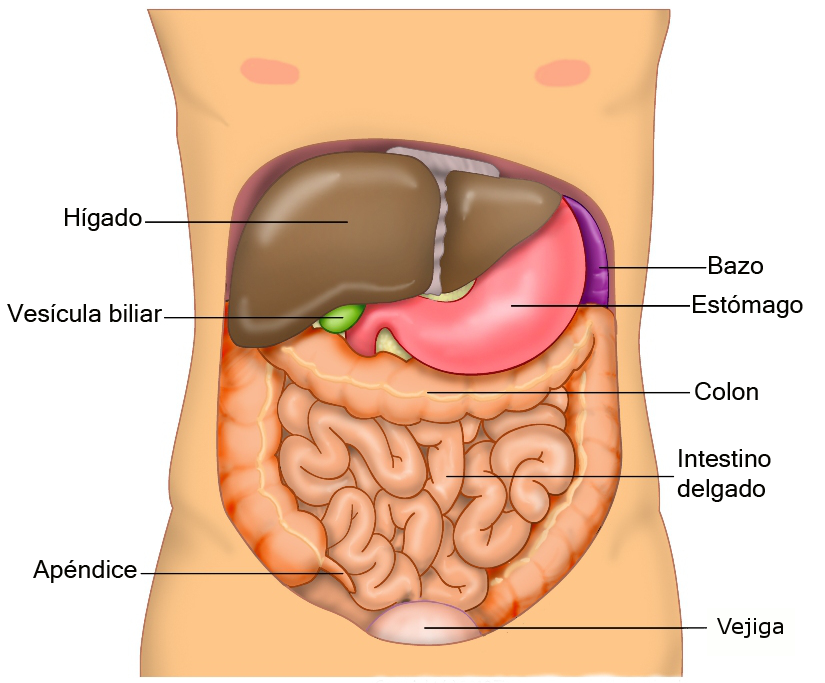
\includegraphics[width=.70\textwidth]{figuras/anatomia_higado.png} \\
\end{center}

Las funciones del hígado son múltiples y diversas. Las principales son procesar, particionar y metabolizar macronutrientes, regular el volumen de sangre, apoyar al sistema inmune, eliminar sustancias químicas como el alcohol y otras drogas y producir bilis para absorber grasas \cite{Trefts2017}. Es un órgano imprescindible para la vida.

\subsubsection{Factores de riesgo}

Uno de los factores de riesgo más comunes del cáncer de hígado es la presencia de cirrosis, o sustitución de células sanas de hígado por tejido cicatrizado. La cirrosis puede producirse por varias causas, siendo las más habituales el consumo excesivo de alcohol y la infección con el virus de la hepatitis B o C \cite{AmericanCancerSociety2019}. Otros factores de riesgo son el tabaco, la obesidad, padecer diabetes tipo II y consumir esteroides anabólicos \cite{AmericanCancerSociety2019, Marrero2005}.\\

La prevención del cáncer de hígado se basa en reducir la exposición a factores de riesgo como el tabaco y el alcohol, y en vacunarse contra la hepatitis B \cite{AmericanCancerSociety2019}.

% ---------------------------------

\subsection{Cáncer de colon-recto}

Las neoplasias malignas de colon, recto, unión rectosigmoidea, ano y canal anal (códigos C18-C21 según la Clasificación Internacional de Enfermedades, Décima Revisión \cite{ICD10, cie10es}) a menudo se estudian agrupadas por tener características muy similares.

\subsubsection{Anatomía y funciones del colon-recto}

El colon tiene 3 funciones principales: absorción de agua y electrolitos, producción y absorción de vitaminas y movimiento de heces hacia el recto para su eliminación por el ano \cite{Azzouz2020}.\\

\textbf{Figura 2}. Anatomía del intestino humano. Ilustración de Ties van Brussel.
\begin{center}
	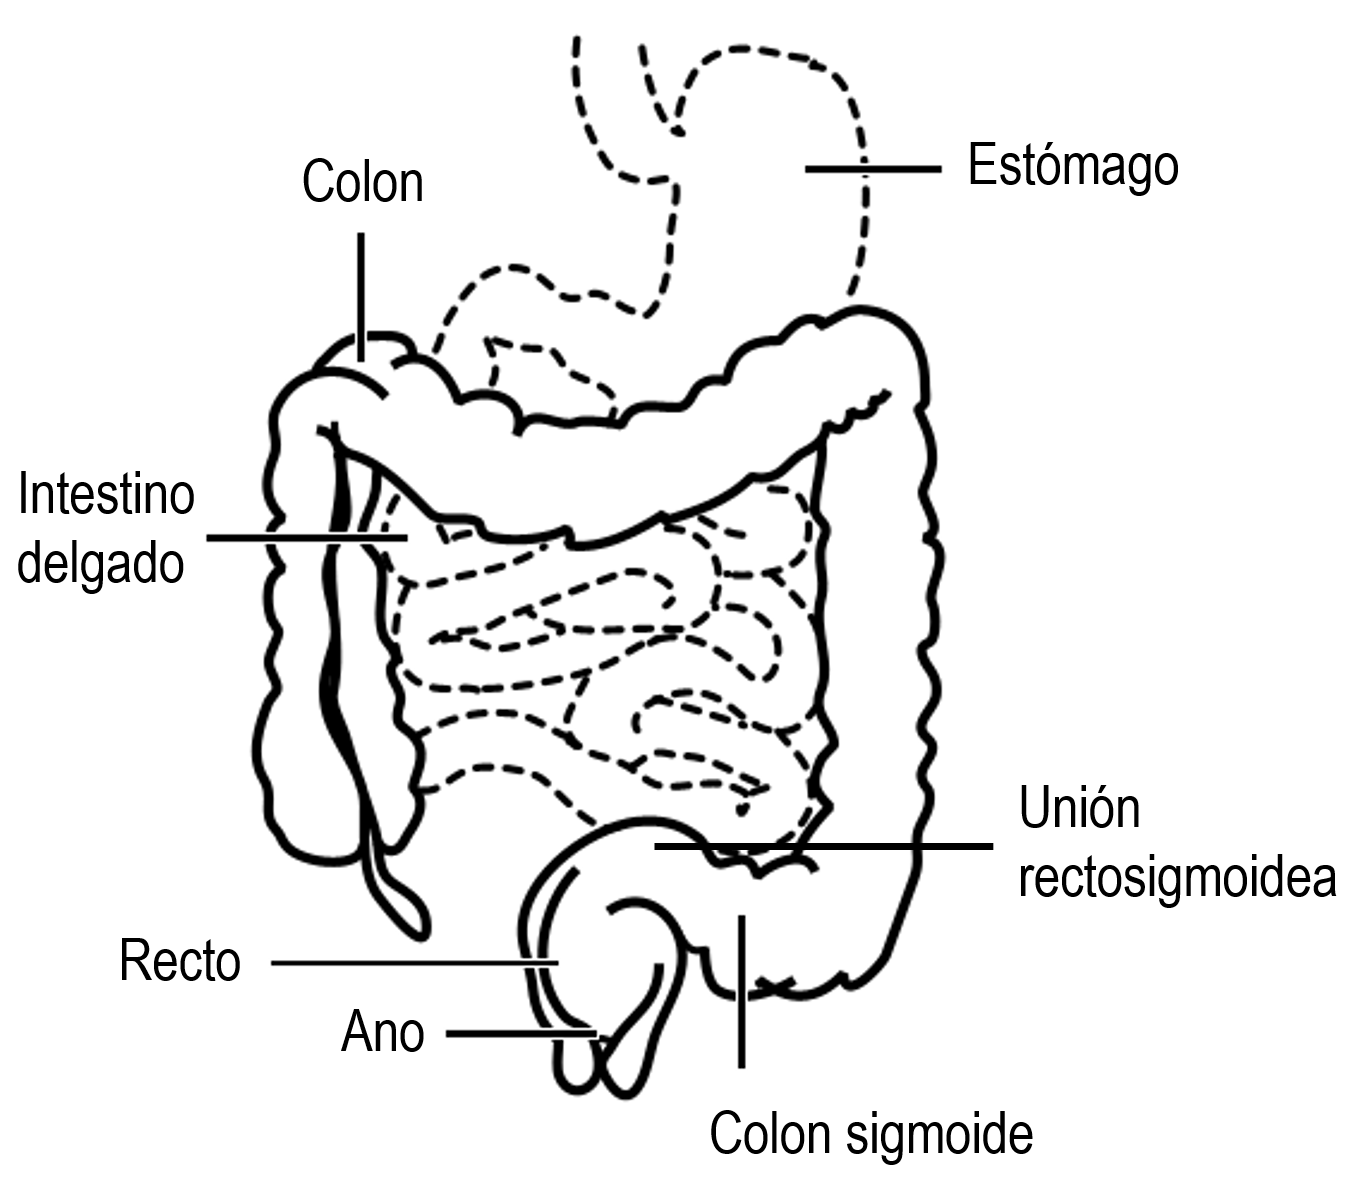
\includegraphics[width=.70\textwidth]{figuras/anatomia_cr.png} \\
\end{center}

\subsubsection{Factores de riesgo}

Entre los factores de riesgo del cáncer de colon-recto se puede distinguir entre factores modificables y no modificables.\\

Entre los factores de riesgo que son modificables destacan el sobrepeso, la inactividad física, las dietas con alto consumo de carnes rojas o procesadas, y el consumo de tabaco y alcohol \cite{AmericanCancerSociety2020}.\\

Una edad superior a 50 años, padecer diabetes tipo 2 y tener antecedentes personales o familiares de cáncer de colon-recto, pólipos o enfermedad intestinal inflamatoria, como colitis ulcerosa y enfermedad de Crohn, son algunos de los factores de riesgo no modificables \cite{AmericanCancerSociety2020}. También existen algunos síndromes hereditarios como el síndrome de Lynch que aumentan las posibilidades de padecer cáncer de colon-recto \cite{Lynch2003}.\\

Para intentar prevenir el cáncer de colon-recto se deben cambiar aquellos factores que son modificables: realizar ejercicio, mantener una dieta saludable y evitar el consumo de tabaco y alcohol. Además, en los últimos años se están implementando programas de cribado de cáncer de colon-recto para detectar pólipos o diagnosticar el cáncer en etapas iniciales mediante análisis como pruebas de sangre oculta en heces o colonoscopias \cite{Levin2008}.\\

% ---------------------------------

\section{Ciencias -ómicas}

\textcolor{red}{Principales con descripción + mencionar otras}

\textcolor{red}{Ver apuntes asignatura bioinformática}

\subsection{¿Secuenciación del genoma?}

\textcolor{red}{Human Genome Project, ...}

\textcolor{red}{DEGs, }

\subsection{Transcriptómica y ARN}

\textcolor{red}{Daniel: La
	genómica estudia el genoma como tal (Cromosomas, mutaciones y
	variaciones tanto de nucleótidos concretos como de regiones del genoma),
	sin embargo la transcriptómica estudia las transcripciones de los genes,
	transcripciones que luego son convertidas a proteínas. Tanto RNA-seq
	como microRNA, se enmarcan en el ámbito de transcriptómica.}



	
	% Epidemiología del cáncer
	\chapter{Epidemiología del cáncer}

La Epidemiología se ha definido tradicionalmente como la ciencia que estudia la distribución y los determinantes de la enfermedad en los seres humanos \cite{MacMahon1970}. En una definición más moderna, no limitada exclusivamente a la enfermedad, la Epidemiología se define como el estudio de la aparición y distribución de los estados o acontecimientos relacionados con la salud en poblaciones específicas, incluyendo el estudio de los determinantes de estos estados, y la aplicación de este conocimiento al control de los problemas de la salud \cite{Porta2008}.

\section{Indicadores epidemiológicos}

Para medir en la población el impacto del cáncer se utilizan principalmente cuatro indicadores:

\begin{itemize}
	\item \textbf{Incidencia} (casos nuevos). Mide el riesgo de presentar cáncer.
	\item \textbf{Mortalidad} (defunciones). Mide el riesgo de morir por cáncer.
	\item \textbf{Supervivencia} (porcentaje de casos vivos). Mide la historia natural del cáncer y efectividad del tratamiento.
	\item \textbf{Prevalencia} (casos nuevos y antiguos, vivos). Mide la carga asistencial de la enfermedad.
\end{itemize}

Además, se puede examinar la evolución de cada indicador a lo largo del tiempo, hablando así de tendencias de la incidencia, de la mortalidad, de la supervivencia o de la prevalencia.\\

% ---------------------------------

\section{Fuentes de información}

A nivel mundial, las estadísticas de incidencia, mortalidad y prevalencia de cáncer las proporciona el \textit{Global Cancer Observatory} (GCO), una plataforma web de la \textit{International Agency for Research on Cancer}, de la Organización Mundial de la Salud \cite{Bray2018, GCO}. El organismo equivalente al GCO a nivel europeo es el \textit{European Cancer Information System} (ECIS), de reciente creación y apoyado por la Comisión Europea \cite{ECIS, ECIS2}. Para conocer la supervivencia, el programa CONCORD \cite{Allemani2018} publica datos a nivel mundial y EUROCARE \cite{DeAngelis2014} a nivel europeo.\\

Aunque estos organismos proporcionan estadísticas sobre cáncer en España, también existen fuentes a nivel nacional que cuentan con datos más actualizados y con distinta metodología. La Red Española de Registros de Cáncer (REDECAN) publica periódicamente datos sobre incidencia y supervivencia de cáncer en España \cite{REDECAN2020, Guevara2019}, mientras que las estadísticas de mortalidad por cáncer se pueden calcular a partir de las defunciones que publica el Ministerio de Sanidad, Consumo y Bienestar Social (MSCBS) del Gobierno de España \cite{MSCBS} y la población que proporciona el Instituto Nacional de Estadística \cite{INEpob}.\\

% ---------------------------------

\section{Incidencia de cáncer}

\subsection{Metodología}

Para medir de manera precisa la incidencia de cáncer en una población es necesaria la existencia de un Registro de Cáncer Poblacional. Estas entidades se dedican a registrar exhaustivamente todos los casos de cáncer diagnosticados en un área geográfica, y sus datos son muy útiles para todo tipo de estudios epidemiológicos. Algunos de estos Registros cubren la población de todo un país (por ejemplo, Canadá) mientras que otros cubren regiones concretas (por ejemplo, la provincia de Granada). Desgraciadamente, muchas áreas geográficas no están cubiertas por un Registro de Cáncer Poblacional. Es el caso de España, en el que sólo el 27\% de la población está cubierta por un Registro de Cáncer Poblacional \cite{Redondo-Sanchez2019}. Para conocer de manera estimada la incidencia de cáncer en territorios sin Registro de Cáncer Poblacional o proyectar la incidencia a años posteriores se utilizan diversos métodos matemáticos y estadísticos \cite{Bray2018, GCO, ECIS, ECIS2, REDECAN2020, Redondo-Sanchez2019}.\\

Con respecto a las medidas usadas para reportar la incidencia, la más sencilla y fácil de interpretar es el número nuevo de casos de cáncer, enmarcado siempre en un periodo concreto de tiempo y un área geográfica. A partir del número de casos se puede calcular la tasa bruta (TB), un indicador que tiene en cuenta el tamaño de la población y que se suele calcular por 100.000 habitantes \cite{IARC1995}.\\

$$\text{TB}  = 100.000 \cdot \dfrac{\text{Número de casos nuevos}}{\text{Personas-año a riesgo}}$$\\

Para permitir comparaciones entre distintas poblaciones, o la misma población en momentos distintos, es necesario tener en cuenta la estructura de edad de la población. Para responder a esta motivación se define la tasa estandarizada por edad (TE) como aquella tasa que habría en la población de estudio si tuviese exactamente la misma estructura de edad que una población estándar predefinida \cite{IARC1995}. La definición de la tasa estandarizada por edad para 18 grupos de edad quinquenales (0-4 años, 5-9 años, $\dots$, 80-84 años, 85 años y más) es la siguiente:

$$\text{TE} = \sum_{i = 1}^{18} \omega_i \dfrac{N_i}{P_i} $$
donde $N_i$ y $P_i$ son respectivamente el número de casos incidentes y la población en el $i$-ésimo grupo de edad, y $\omega_i$ es el peso que toma la población de referencia en el grupo $i$-ésimo, con $\sum_{i = 1}^{18}\omega_i = 100.000$. Los valores de ${\omega_i}$ están predefinidos en base a poblaciones estándar, siendo las más utilizadas en nuestro contexto las siguientes:

\begin{itemize}
	
	\item Población mundial. Propuesta por primera vez en 1960 \cite{SegiM.1960} y modificada más tarde en 1966 \cite{Doll1966}, permite realizar comparaciones a nivel mundial.
		
	\item Antigua población estándar europea. Propuesta en 1976 \cite{Waterhouse1976} basándose en la estructura de edad de varias poblaciones escandinavas, permite comparaciones entre zonas europeas.
	
	\item Nueva población estándar europea. En el año 2013, la Oficina Europea de Estadística (EUROSTAT) realiza una revisión de la población estándar europea con el objetivo de que la población refleje fielmente el envejecimiento existente en la población europea \cite{EUROSTAT2013}. Debido a su novedad, el uso de esta población aún no está ampliamente extendido en los organismos internacionales \cite{ECIS2} y en ocasiones se reportan las dos tasas estandarizadas por las poblaciones estándar antigua y nueva \cite{ECIS}.
	

\end{itemize}

En la Tabla 1 se muestran los pesos para cada una de las poblaciones de referencia mencionadas anteriormente.\\

%\newpage
\textbf{Tabla 1}. Pesos de las poblaciones estándar para el cálculo de tasas estandarizadas por edad.
\begin{table}[!htb]
	\begin{tabular}{|r|r|r|r|}
		\hline		
		Grupo de edad  &  \begin{tabular}[r]{@{}r@{}}Población estándar\\ mundial\end{tabular}  &  \begin{tabular}[r]{@{}r@{}}Población estándar\\ europea 1976\end{tabular}  &  \begin{tabular}[r]{@{}r@{}}Población estándar\\ europea 2013\end{tabular}\\\hline
		
		0-4 años  &  12.000  &  8.000  &  5.000\\
		5-9 años  &  10.000  &  7.000  &  5.500\\
		10-14 años  &  9.000  &  7.000  &  5.500\\
		15-19 años  &  9.000  &  7.000  &  5.500\\
		20-24 años  &  8.000  &  7.000  &  6.000\\
		25-29 años  &  8.000  &  7.000  &  6.000\\
		30-34 años  &  6.000  &  7.000  &  6.500\\
		35-39 años  &  6.000  &  7.000  &  7.000\\
		40-44 años  &  6.000  &  7.000  &  7.000\\
		45-49 años  &  6.000  &  7.000  &  7.000\\
		50-54 años  &  5.000  &  7.000  &  7.000\\
		55-59 años  &  4.000  &  6.000  &  6.500\\
		60-64 años  &  4.000  &  5.000  &  6.000\\
		65-69 años  &  3.000  &  4.000  &  5.500\\
		70-74 años  &  2.000  &  3.000  &  5.000\\
		75-79 años  &  1.000  &  2.000  &  4.000\\
		80-84 años  &  500  &  1.000  &  2.500\\
		$\geq$85 años  &  500  &  1.000  &  2.500\\\hline
	\end{tabular}
\end{table}

Para utilizar notación internacional, la tasa estandarizada por la población mundial se notará TE-M (población mundial), la tasa estandarizada por la población europea de 1976 se notará TE-aE (antigua población europea) y la de 2013 se notará TE-nE (nueva población europea).

\subsection{Incidencia del total del cáncer excepto piel no melanoma}

El cáncer de piel no melanoma se suele excluir al reportar datos de incidencia del total del cáncer, debido a que es muy frecuente y cuenta con buen pronóstico, por lo que no se suele registrar en los Registros de Cáncer Poblacionales \cite{Gordon2013, Madan2010}.\\

Para dar una perspectiva global del cáncer y sus diferentes tipos, en la Figura 3 se muestran las localizaciones anatómicas más frecuentes de cáncer en el mundo, así como su distribución por sexos.\\

%\newpage
\textbf{Figura 3}. Gráfico de mosaico con la incidencia estimada de cáncer excepto piel no melanoma en el mundo para el año 2018. Ocho localizaciones anatómicas más frecuentes en ambos sexos. Fuente: \textit{Global Cancer Observatory}, Organización Mundial de la Salud \cite{GCO}.
\begin{center}
	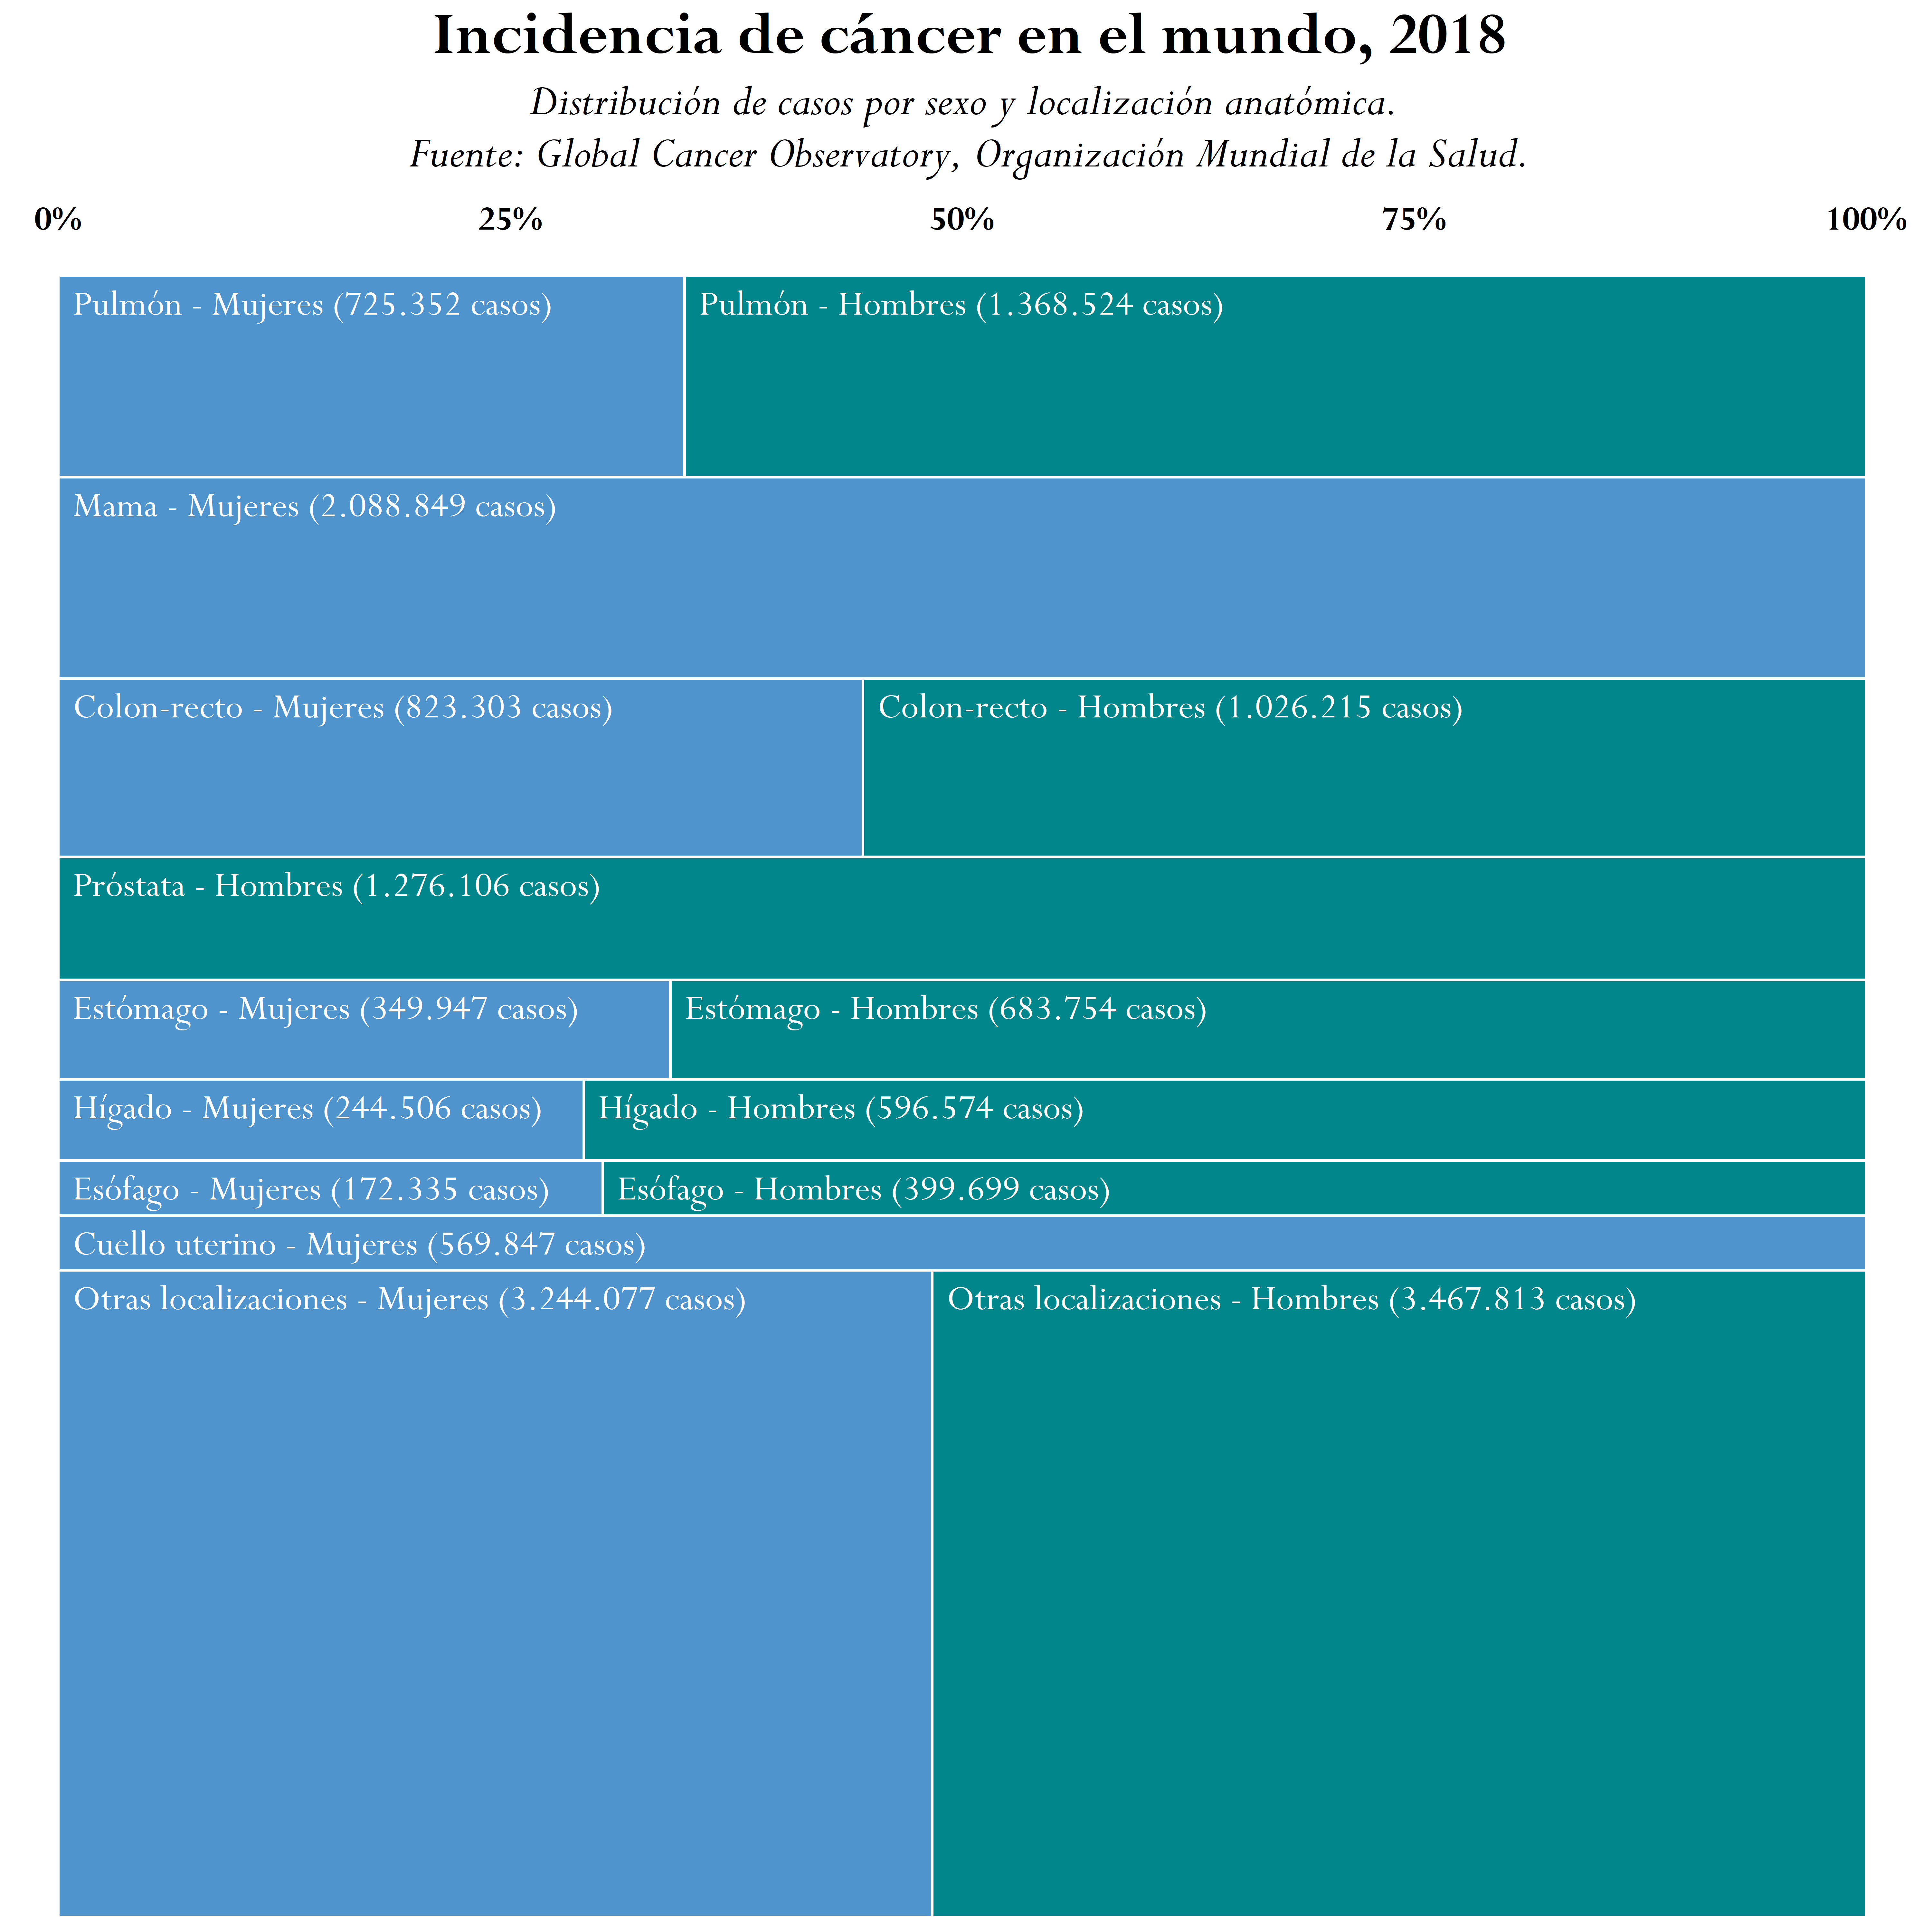
\includegraphics[width=1\textwidth]{figuras/marimekko_gco_incidencia.png} \\
\end{center}

El cáncer de pulmón es el más frecuente en todo el mundo, seguido por los cánceres de mama, colon-recto, próstata, estómago, hígado, esófago y cuello uterino. En la mayoría de las localizaciones anatómicas el cáncer es más frecuente en hombres que en mujeres (Figura 3).\\

%\newpage
\textbf{Tabla 2}. Incidencia del total del cáncer excepto piel no melanoma en 2018, por sexo y población. Número de casos nuevos (N), tasa bruta (TB), tasa estandarizada por la población mundial (TE-M),  tasa estandarizada por la antigua población europea (TE-aE) y  tasa estandarizada por la nueva población europea (TE-nE).

\begin{table}[H]
	\begin{tabular}{|c|l|c|r|r|r|r|r|}
		\hline		

		\multicolumn{1}{|c|}{Sexo} & \multicolumn{1}{|c|}{Población} & Fuente & \multicolumn{1}{|c|}{N} & \multicolumn{1}{|c|}{TB} & \multicolumn{1}{|c|}{TE-M} & \multicolumn{1}{|c|}{TE-aE} & \multicolumn{1}{|c|}{TE-nE}\\\hline
		
		\multirow{3}{*}{Hombres} & Mundo & GCO \cite{GCO} & 8.818.685 & 229,0 & 204,7 &  & \\
		& Europa & ECIS \cite{ECIS} & 2.059.673 & 572,9 & 302,7 & 436,0 & 651,7\\
		& España & ECIS \cite{ECIS} & 142.353 & 625,6 & 309,7 & 444,7 & 658,6\\\hline
		\multirow{3}{*}{Mujeres} & Mundo & GCO \cite{GCO} & 8.218.216 & 217,3 & 175,6 &  & \\
		& Europa & ECIS \cite{ECIS} & 1.851.644 & 481,8 & 242,7 & 332,6 & 451,2\\
		& España & ECIS \cite{ECIS} & 106.647 & 451,1 & 218,4 & 298,5 & 401,7\\\hline
		\multirow{3}{*}{\begin{tabular}[c]{@{}c@{}}Ambos\\sexos\end{tabular}} & Mundo & GCO \cite{GCO} & 17.036.901 & 223,2 & 187,8 &  & \\
		& Europa & ECIS \cite{ECIS} & 3.911.317 & 525,8 & 266,7 & 374,3 & 531,9\\
		& España & ECIS \cite{ECIS} & 249.000 & 536,7 & 259,4 & 363,8 & 515,3\\\hline
	\end{tabular}
\end{table}

A nivel nacional, REDECAN ha publicado estimaciones de la incidencia en España más recientes a las mostradas en la Tabla 2, correspondientes al año 2020, \cite{REDECAN2020}. En este análisis se estima el número de casos de cáncer excepto piel no melanoma en 277.394 casos (57,8\% en hombres), con una tasa bruta de 588,0 por 100.000 habitantes y tasas estandarizadas de 280,3 (TE-M), 399,4 (TE-aE) y 579,8 (TE-nE).

\subsection{Incidencia de cáncer de hígado}

El cáncer de hígado es el sexto cáncer más frecuente del mundo (Figura 3), con más de 840.000 casos nuevos anuales en todo el mundo, 82.000 de ellos en Europa y 6.600 en España (Tabla 3). Es un cáncer más frecuente en hombres que en mujeres: por cada caso en mujeres hay 2,4 casos en hombres. En ambos sexos, la TE-M de España (6,5) es mayor que la de Europa (5,1) aunque mucho menor que la del mundo (9,3).\\

\newpage
\textbf{Tabla 3}. Incidencia de cáncer de hígado en 2018, por sexo y población. Número de casos nuevos (N), tasa bruta (TB), tasa estandarizada por la población mundial (TE-M),  tasa estandarizada por la antigua población europea (TE-aE) y  tasa estandarizada por la nueva población europea (TE-nE).

\begin{table}[H]
	\begin{tabular}{|c|l|c|r|r|r|r|r|}
		\hline		
		
		\multicolumn{1}{|c|}{Sexo} & \multicolumn{1}{|c|}{Población} & Fuente & \multicolumn{1}{|c|}{N} & \multicolumn{1}{|c|}{TB} & \multicolumn{1}{|c|}{TE-M} & \multicolumn{1}{|c|}{TE-aE} & \multicolumn{1}{|c|}{TE-nE}\\\hline
		
		\multirow{3}{*}{Hombres} & Mundo & GCO \cite{GCO} & 596.574 & 15,5 & 13,9 &  & \\
		& Europa & ECIS \cite{ECIS} & 55.825 & 15,5 & 8,0 & 11,7 & 17,7\\
		& España & ECIS \cite{ECIS} & 4.976 & 21,9 & 10,9 & 15,7 & 22,5\\\hline
		\multirow{3}{*}{Mujeres} & Mundo & GCO \cite{GCO} & 244.506 & 6,5 & 4,9 &  & \\
		& Europa & ECIS \cite{ECIS} & 26.641 & 6,9 & 2,7 & 4,0 & 6,3\\
		& España & ECIS \cite{ECIS} & 1.654 & 7,0 & 2,4 & 3,6 & 6,0\\\hline
		\multirow{3}{*}{\begin{tabular}[c]{@{}c@{}}Ambos\\sexos\end{tabular}} & Mundo & GCO \cite{GCO} & 841.080 & 11,0 & 9,3 &  & \\
		& Europa & ECIS \cite{ECIS} & 82.466 & 11,1 & 5,1 & 7,4 & 11,3\\
		& España & ECIS \cite{ECIS} & 6.630 & 14,3 & 6,5 & 9,3 & 13,6\\\hline
				
	\end{tabular}
\end{table}

En las estimaciones publicadas por REDECAN para 2020 se estiman en España 6.595 casos de cáncer de hígado (75,4\% en hombres), con una tasa bruta de 14,0 y tasas estandarizadas de 6,5 (TE-M), 9,4 (TE-aE) y 13,9 (TE-nE) \cite{REDECAN2020}.

\subsection{Incidencia de cáncer de colon-recto}

El cáncer de colon-recto es el tercer cáncer más frecuente del mundo (Figura 3), con más de 1.800.000 casos nuevos anuales en todo el mundo. En Europa y España es el cáncer más frecuente en ambos sexos con 510.000 casos anuales en Europa y 37.000 en España (Tabla 4). Es un cáncer ligeramente más frecuente en hombres que en mujeres: por cada caso en mujeres hay 1,2 casos en hombres. En ambos sexos, la TE-M de España (81,1) es mayor que la de Europa (68,8) y la del mundo (24,2), lo que puede deberse a una mayor exposición a factores de riesgo como el tipo de dieta o la ausencia de un programa de cribado a nivel nacional \cite{Zavoral2009}.\\

\textbf{Tabla 4}. Incidencia de cáncer de colon-recto en 2018, por sexo y población. Número de casos nuevos (N), tasa bruta (TB), tasa estandarizada por la población mundial (TE-M),  tasa estandarizada por la antigua población europea (TE-aE) y  tasa estandarizada por la nueva población europea (TE-nE).

\begin{table}[H]
	\begin{tabular}{|c|l|c|r|r|r|r|r|}
		\hline		
		
		\multicolumn{1}{|c|}{Sexo} & \multicolumn{1}{|c|}{Población} & Fuente & \multicolumn{1}{|c|}{N} & \multicolumn{1}{|c|}{TB} & \multicolumn{1}{|c|}{TE-M} & \multicolumn{1}{|c|}{TE-aE} & \multicolumn{1}{|c|}{TE-nE}\\\hline
		
		\multirow{3}{*}{Hombres} & Mundo & GCO \cite{GCO} & 1.026.215 & 26,6 & 23,6 &  & \\
		& Europa & ECIS \cite{ECIS} & 275.519 & 76,6 & 38,1 & 56,8 & 88,9\\
		& España & ECIS \cite{ECIS} & 23.013 & 101,1 & 45,8 & 68,5 & 107,2\\\hline
		\multirow{3}{*}{Mujeres} & Mundo & GCO \cite{GCO} & 823.303 & 21,8 & 16,3 &  & \\
		& Europa & ECIS \cite{ECIS} & 236.101 & 61,4 & 25,2 & 37,0 & 56,3\\
		& España & ECIS \cite{ECIS} & 14.642 & 61,9 & 23,6 & 34,9 & 53,5\\\hline
		\multirow{3}{*}{\begin{tabular}[c]{@{}c@{}}Ambos\\sexos\end{tabular}} & Mundo & GCO \cite{GCO} & 1.849.518 & 24,2 & 19,7 &  & \\
		& Europa & ECIS \cite{ECIS} & 511.620 & 68,8 & 30,8 & 45,6 & 70,0\\
		& España & ECIS \cite{ECIS} & 37.655 & 81,1 & 33,9 & 50,4 & 77,5\\\hline
	\end{tabular}
\end{table}

En las estimaciones publicadas por REDECAN para 2020 se estiman en España 44.231 casos de cáncer de colon-recto (58,9\% en hombres), con una tasa bruta de 93,8 y tasas estandarizadas de 40,0 (TE-M), 59,5 (TE-aE) y 91,9 (TE-nE) \cite{REDECAN2020}.

% ---------------------------------

\section{Mortalidad por cáncer}

\subsection{Metodología}

Los indicadores para medir la mortalidad por cáncer son los mismos que para la incidencia, cambiando número de casos por defunciones por cáncer. Es importante destacar que la mortalidad por cáncer es por definición aquella mortalidad que es causada directamente por el cáncer. En este sentido, una persona diagnosticada de cáncer que falleciese por otras causas no puede ser considerada como fallecida por cáncer, sino fallecida con cáncer.\\

Aunque ECIS \cite{ECIS} reporta mortalidad por cáncer en España para el año 2018, la mortalidad que se presenta a continuación a nivel nacional es la que proporciona el MSCBS del Gobierno de España \cite{MSCBS}, al tratarse de datos observados basados en certificados médicos de defunción y no estimaciones, por lo que se consideran datos más fiables.
 
\subsection{Mortalidad del total del cáncer excepto piel no melanoma}

En el mundo se producen más de 9 millones de defunciones por cáncer anualmente, siendo esta enfermedad la segunda causa de muerte a nivel global, por detrás de las enfermedades cardiovasculares. Una de cada 6 muertes es causa directa del cáncer \cite{WorldHealthOrganization2018}.\\

En ambos sexos, los cánceres que provocan más defunciones son los de pulmón, colon-recto y estómago, mientras que en mujeres el cáncer con más defunciones es el cáncer de mama y en hombres el de pulmón (Figura 4).\\

\textbf{Figura 4}. Gráfico de mosaico con la mortalidad estimada por cáncer excepto piel no melanoma en el mundo para el año 2018. Ocho localizaciones anatómicas con más defunciones en ambos sexos. Fuente: \textit{Global Cancer Observatory}, Organización Mundial de la Salud \cite{GCO}.
\begin{center}
	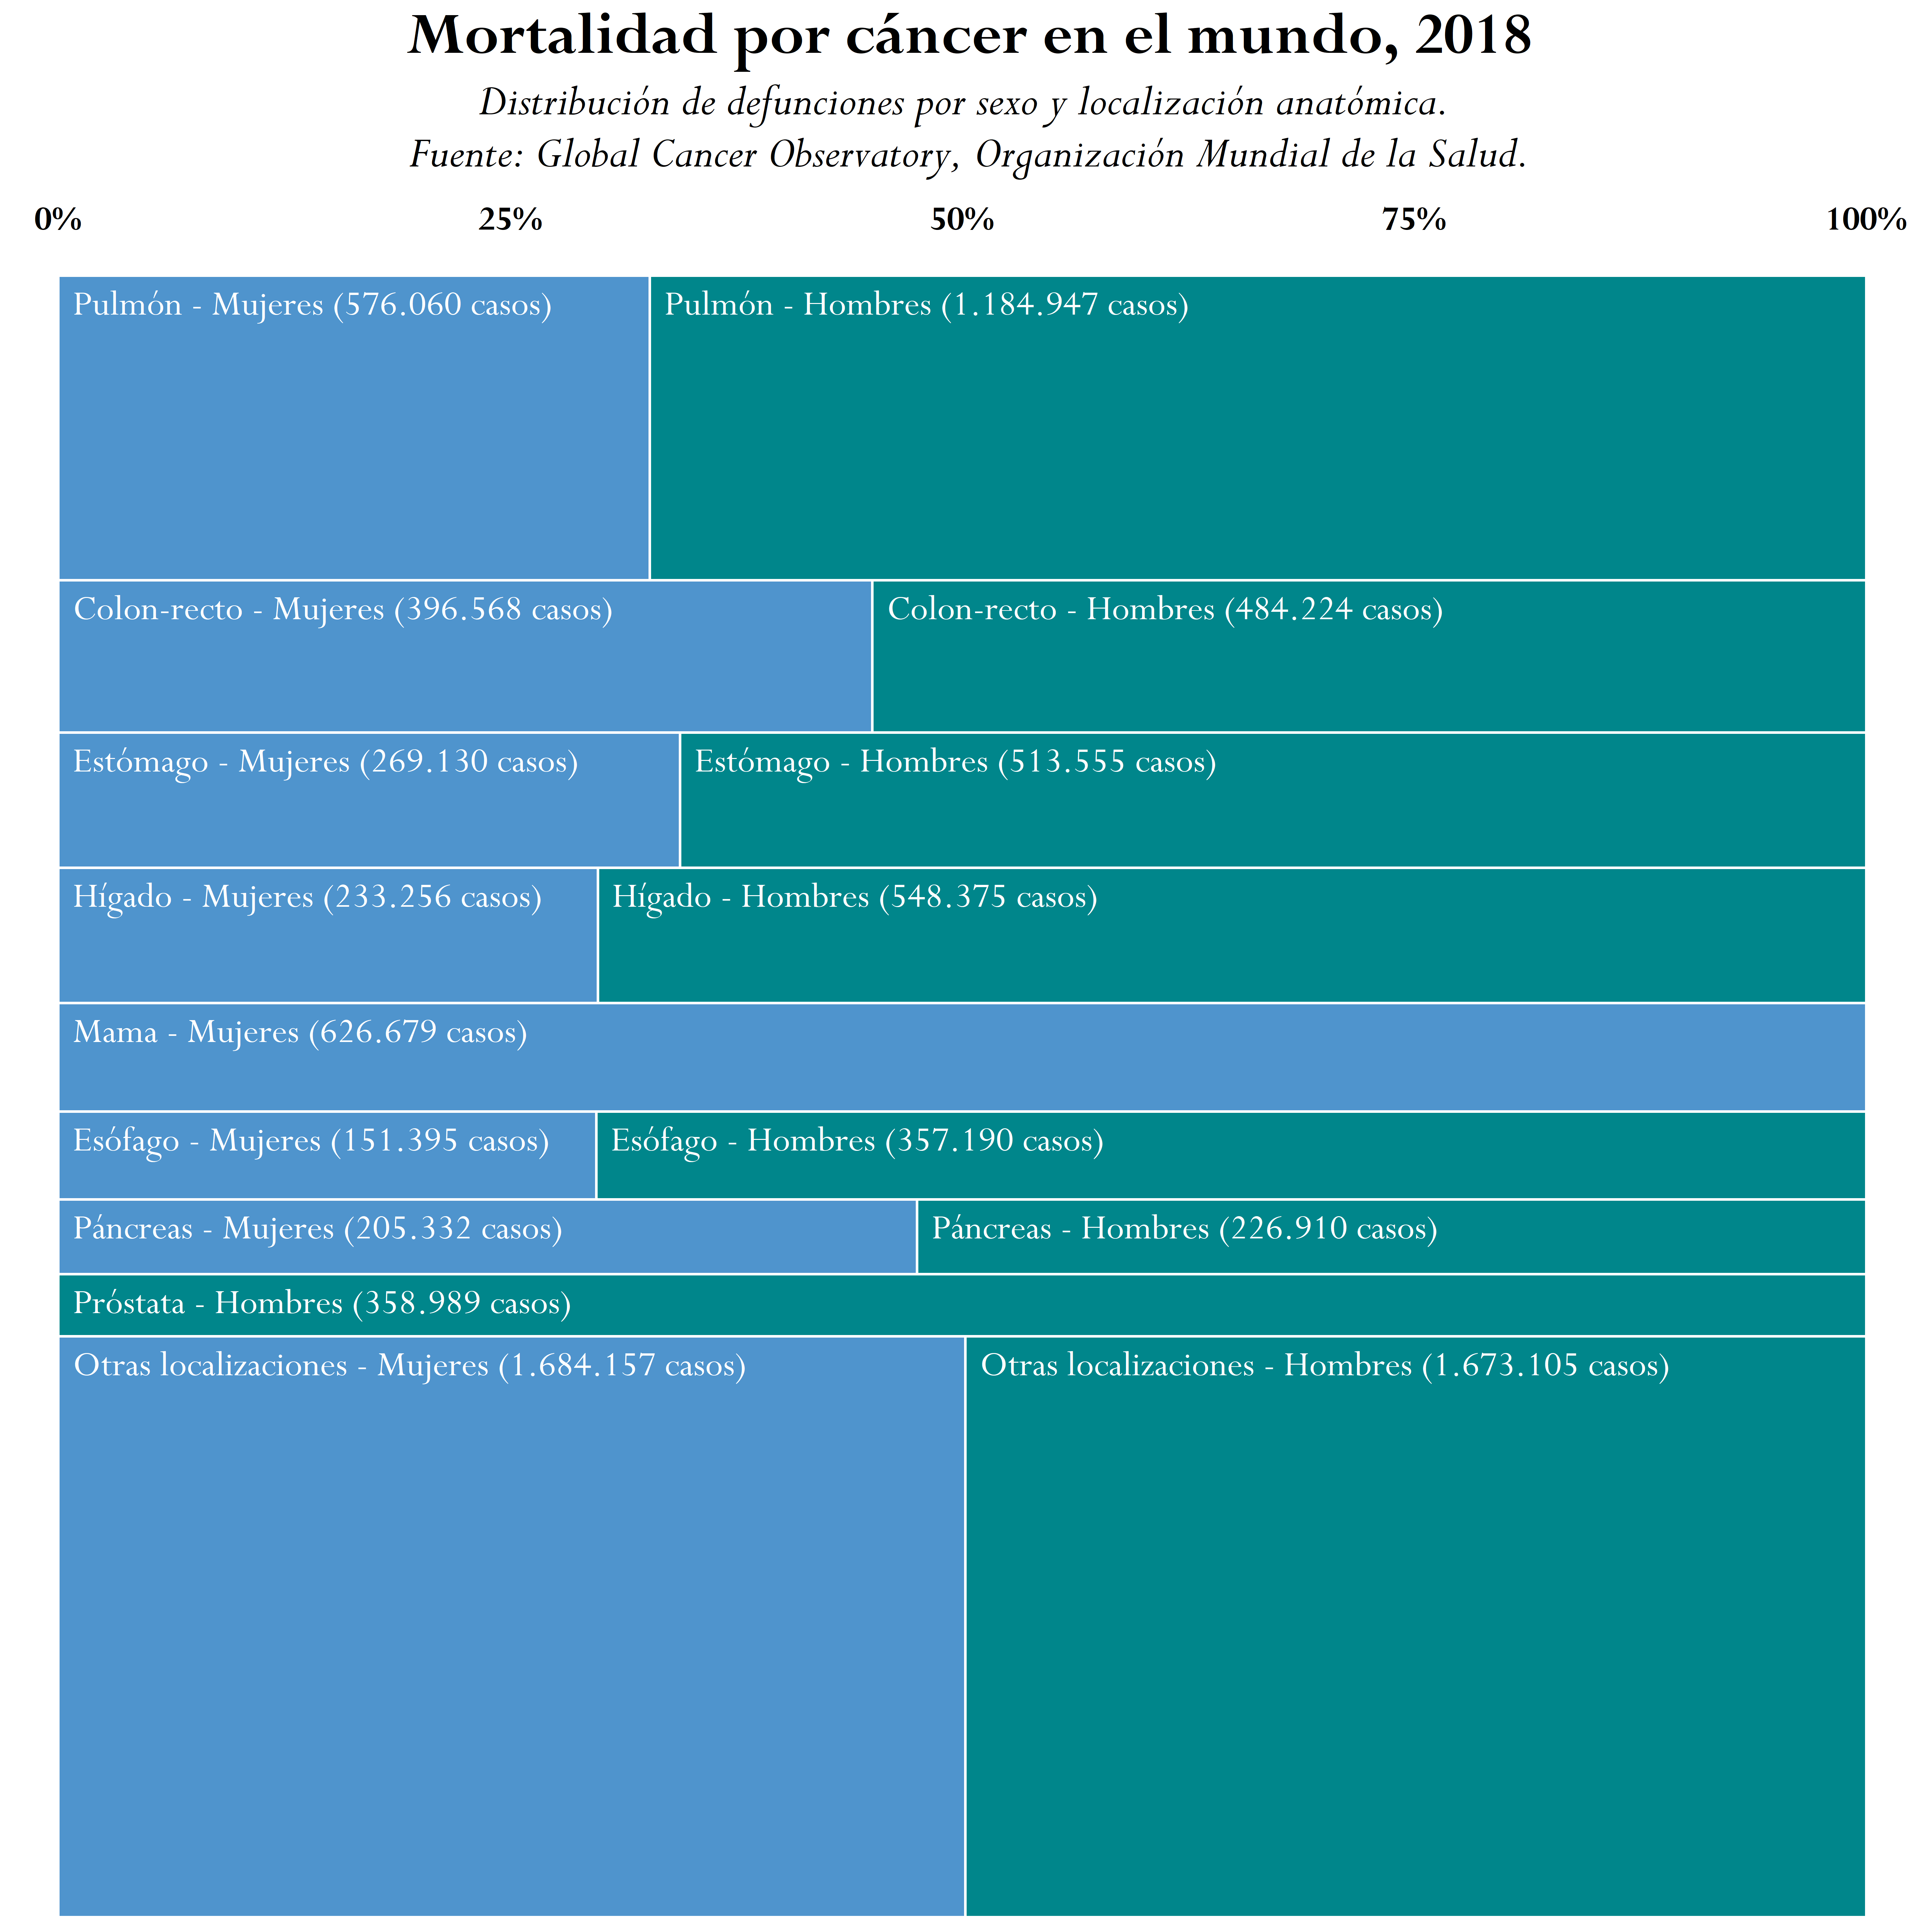
\includegraphics[width=1\textwidth]{figuras/marimekko_gco_mortalidad.png} \\
\end{center}

En España se producen más de 100.000 muertes anuales por cáncer, siendo la tasa de mortalidad inferior a la europea y a la mundial tanto en ambos sexos como en hombres y mujeres (Tabla 5).\\

\textbf{Tabla 5}. Mortalidad por total del cáncer excepto piel no melanoma en 2018, por sexo y población. Número de defunciones (N), tasa bruta (TB), tasa estandarizada por la población mundial (TE-M),  tasa estandarizada por la antigua población europea (TE-aE) y  tasa estandarizada por la nueva población europea (TE-nE).

\begin{table}[H]
	\begin{tabular}{|c|l|r|r|r|r|r|r|}
		\hline		
		
		\multicolumn{1}{|c|}{Sexo} & \multicolumn{1}{|c|}{Población} & \multicolumn{1}{|c|}{Fuente} & \multicolumn{1}{|c|}{N} & \multicolumn{1}{|c|}{TB} & \multicolumn{1}{|c|}{TE-M} & \multicolumn{1}{|c|}{TE-aE} & \multicolumn{1}{|c|}{TE-nE}\\\hline
		
		\multirow{3}{*}{Hombres} & Mundo & GCO \cite{GCO} & 5.347.295 & 138,9 & 121,9 &  & \\
		& Europa & ECIS \cite{ECIS} & 1.077.986 & 299,8 & 143,2 & 217,4 & 355,4\\
		& España & MSCBS \cite{MSCBS} & 65.610 & 286,4 & 121,3 & 186,8 & 314,1\\\hline
		\multirow{3}{*}{Mujeres} & Mundo & GCO \cite{GCO} & 4.142.577 & 109,5 & 82,7 &  & \\
		& Europa & ECIS \cite{ECIS} & 851.723 & 221,6 & 86,4 & 128,1 & 201,0\\
		& España & MSCBS \cite{MSCBS} & 42.248 & 177,4 & 63,2 & 94,6 & 151,1\\\hline
		\multirow{3}{*}{\begin{tabular}[c]{@{}c@{}}Ambos\\sexos\end{tabular}} & Mundo & GCO \cite{GCO} & 9.489.872 & 124,3 & 100,5 &  & \\
		& Europa & ECIS \cite{ECIS} & 1.929.709 & 259,4 & 110,8 & 165,8 & 263,9\\
		& España & MSCBS \cite{MSCBS} & 107.858 & 230,8 & 89,4 & 135,4 & 221,2\\\hline

	\end{tabular}
\end{table}


\subsection{Mortalidad de cáncer de hígado}

Si bien el cáncer de hígado es el sexto cáncer más incidente del mundo, en mortalidad ocupa la cuarta posición, siendo la causa de 782.000 defunciones anuales (Figura 4). La muerte por cáncer de hígado es mucho más frecuente en hombres que en mujeres. En Europa el cáncer de hígado causa cerca de 80.000 muertes y en España unas 5.100, con unas tasas de mortalidad muy similares y por debajo de la tasa mundial (Tabla 6).\\

\textbf{Tabla 6}. Mortalidad por cáncer de hígado en 2018, por sexo y población. Número de defunciones (N), tasa bruta (TB), tasa estandarizada por la población mundial (TE-M),  tasa estandarizada por la antigua población europea (TE-aE) y  tasa estandarizada por la nueva población europea (TE-nE).


\begin{table}[H]
	\begin{tabular}{|c|l|r|r|r|r|r|r|}
		\hline		
		\multicolumn{1}{|c|}{Sexo} & \multicolumn{1}{|c|}{Población} & \multicolumn{1}{|c|}{Fuente} & \multicolumn{1}{|c|}{N} & \multicolumn{1}{|c|}{TB} & \multicolumn{1}{|c|}{TE-M} & \multicolumn{1}{|c|}{TE-aE} & \multicolumn{1}{|c|}{TE-nE}\\\hline
		
		\multirow{3}{*}{Hombres} & Mundo & GCO \cite{GCO} & 548.375 & 14,2 & 12,7 &  & \\
		& Europa & ECIS \cite{ECIS} & 50.365 & 14,0 & 6,8 & 10,3 & 16,4\\
		& España & MSCBS \cite{MSCBS} & 3.577 & 15,6 & 7,0 & 10,7 & 17,0\\\hline
		\multirow{3}{*}{Mujeres} & Mundo & GCO \cite{GCO} & 233.256 & 6,2 & 4,6 &  & \\
		& Europa & ECIS \cite{ECIS} & 27.010 & 7,0 & 2,4 & 3,8 & 6,3\\
		& España & MSCBS \cite{MSCBS} & 1.564 & 6,6 & 2,0 & 3,2 & 5,6\\\hline
		\multirow{3}{*}{\begin{tabular}[c]{@{}c@{}}Ambos\\sexos\end{tabular}} & Mundo & GCO \cite{GCO} & 781.631 & 10,2 & 8,5 &  & \\
		& Europa & ECIS \cite{ECIS} & 77.375 & 10,4 & 4,4 & 6,6 & 10,6\\
		& España & MSCBS \cite{MSCBS} & 5.141 & 11,0 & 4,4 & 6,7 & 10,7\\\hline

		
	\end{tabular}
\end{table}

\subsection{Mortalidad de cáncer de colon-recto}

El cáncer de colon-recto es el segundo cáncer que provoca más defunciones, con más de 880.000 defunciones anuales en todo el mundo (Figura 4). La defunción por cáncer de colon-recto es ligeramente más frecuente en hombres que en mujeres. Las tasas de mortalidad en España y Europa son muy similares, por encima en ambos casos de la tasa mundial (Tabla 7).\\

\textbf{Tabla 7}. Mortalidad por cáncer de colon-recto en 2018, por sexo y población. Número de defunciones (N), tasa bruta (TB), tasa estandarizada por la población mundial (TE-M),  tasa estandarizada por la antigua población europea (TE-aE) y  tasa estandarizada por la nueva población europea (TE-nE).


\begin{table}[H]
	\begin{tabular}{|c|l|r|r|r|r|r|r|}
		\hline		
		
		\multicolumn{1}{|c|}{Sexo} & \multicolumn{1}{|c|}{Población} & \multicolumn{1}{|c|}{Fuente} & \multicolumn{1}{|c|}{N} & \multicolumn{1}{|c|}{TB} & \multicolumn{1}{|c|}{TE-M} & \multicolumn{1}{|c|}{TE-aE} & \multicolumn{1}{|c|}{TE-nE}\\\hline
		
		\multirow{3}{*}{Hombres} & Mundo & GCO \cite{GCO} & 484.224 & 12,6 & 10,8 &  & \\
		& Europa & ECIS \cite{ECIS} & 131.155 & 36,5 & 16,4 & 25,7 & 44,3\\
		& España & MSCBS \cite{MSCBS} & 9.222 & 40,3 & 15,8 & 25,1 & 44,4\\\hline
		\multirow{3}{*}{Mujeres} & Mundo & GCO \cite{GCO} & 396.568 & 10,5 & 7,2 &  & \\
		& Europa & ECIS \cite{ECIS} & 115.059 & 29,9 & 10,0 & 15,6 & 26,6\\
		& España & MSCBS \cite{MSCBS} & 6.066 & 25,5 & 7,5 & 11,9 & 20,7\\\hline
		\multirow{3}{*}{\begin{tabular}[c]{@{}c@{}}Ambos\\sexos\end{tabular}} & Mundo & GCO \cite{GCO} & 880.792 & 11,5 & 8,9 &  & \\
		& Europa & ECIS \cite{ECIS} & 246.214 & 33,1 & 12,8 & 19,9 & 33,8\\
		& España & MSCBS \cite{MSCBS} & 15.288 & 32,7 & 11,2 & 17,7 & 30,9\\\hline
	
	\end{tabular}
\end{table}

% ---------------------------------


\section{Supervivencia de cáncer} 

El proyecto CONCORD (\textit{Global surveillance of cancer survival}), coordinado por la \textit{London School of Hygiene \& Tropical Medicine}, es el mayor proyecto de investigación sobre supervivencia a nivel mundial. En su tercera y última publicación, se analizaron datos de más de 37 millones de pacientes procedentes de 322 Registros de Cáncer Poblacionales de 71 países \cite{Allemani2018}. Las tendencias de la supervivencia están aumentando con el tiempo, aunque se aprecian importantes diferencias entre territorios. Para casos de España diagnosticados durante el periodo 2010-2014, la supervivencia relativa estandarizada por edad a 5 años del diagnóstico es del 63,2\% para cáncer de colon, 59,5\% para cáncer de recto y 17,3\% para cáncer de hígado \cite{Allemani2018}.\\

En el contexto europeo, EUROCARE (\textit{European Cancer Registry based study on survival and care of cancer patients}) proporciona datos para el periodo 2000-2007, estimando la supervivencia relativa estandarizada por edad a 5 años del total del cáncer en un 50,3\% para hombres y 58,0\% para mujeres \cite{DeAngelis2014,ECIS}. Para cáncer de colon-recto la supervivencia es similar a la media global (54,7\% en hombres, 56,7\% en mujeres), y para cáncer de hígado la supervivencia es muy baja (11,5\% tanto para hombres como para mujeres) \cite{DeAngelis2014,ECIS}.\\

REDECAN \cite{Guevara2019}


% ---------------------------------

\section{Prevalencia de cáncer}

\newpage
\textbf{Tabla 8}. Prevalencia del total del cáncer excepto piel no melanoma, cáncer de hígado y cáncer de colon-recto en 2018, por sexo y población. Número de casos prevalentes y tasas por 100.000 habitantes a 1 y 5 años.

\begin{table}[H]
	\begin{tabular}{|c|c|c|rr|rr|}
		%\cline{4-7}
		\hline
		
			 &  &  & \multicolumn{2}{c}{1 año} & \multicolumn{2}{|c|}{5 años} \\\hline
			 &  &  & \multicolumn{1}{c}{N} & \multicolumn{1}{c|}{Tasa} & \multicolumn{1}{c}{N} & \multicolumn{1}{c|}{Tasa} \\ \hline

\multirow{9}{*}{Total del cáncer*} & \multirow{3}{*}{Hombres} & Mundo & 5.607.801 & 145,6 & 17.895.356 & 464,7\\
&  & Europa & 1.504.232 & 418,4 & 5.086.515 & 1414,7\\
&  & España & 105.599 & 464,0 & 356.427 & 1566,3\\ \cline{2-7}
& \multirow{3}{*}{Mujeres} & Mundo & 5.688.175 & 150,4 & 20.738.064 & 548,3\\
&  & Europa & 1.434.849 & 373,4 & 5.417.680 & 1409,8\\
&  & España & 84.409 & 357,0 & 322.341 & 1363,5\\ \cline{2-7}
& \multirow{3}{*}{\begin{tabular}[c]{@{}c@{}}Ambos\\sexos\end{tabular}} & Mundo & 11.295.976 & 148,0 & 38.633.420 & 506,1\\
&  & Europa & 2.939.081 & 395,1 & 10.504.195 & 1412,2\\
&  & España & 190.008 & 409,5 & 678.768 & 1462,9\\ \hline
\multirow{9}{*}{Hígado} & \multirow{3}{*}{Hombres} & Mundo & 236.669 & 6,1 & 471.525 & 12,2\\
&  & Europa & 21.240 & 5,9 & 39.867 & 11,1\\
&  & España & 1.924 & 8,5 & 3.618 & 15,9\\ \cline{2-7}
& \multirow{3}{*}{Mujeres} & Mundo & 97.621 & 2,6 & 203.685 & 5,4\\
&  & Europa & 9.719 & 2,5 & 18.610 & 4,8\\
&  & España & 580 & 2,5 & 1.102 & 4,7\\ \cline{2-7}
& \multirow{3}{*}{\begin{tabular}[c]{@{}c@{}}Ambos\\sexos\end{tabular}} & Mundo & 334.290 & 4,4 & 675.210 & 8,8\\
&  & Europa & 30.959 & 4,2 & 58.477 & 7,9\\
&  & España & 2.504 & 5,4 & 4.720 & 10,2\\ \hline
\multirow{9}{*}{Colon-recto} & \multirow{3}{*}{Hombres} & Mundo & 749.774 & 19,5 & 2.595.326 & 67,4\\
&  & Europa & 213.233 & 59,3 & 748.455 & 208,2\\
&  & España & 18.059 & 79,4 & 63.593 & 279,5\\ \cline{2-7}
& \multirow{3}{*}{Mujeres} & Mundo & 606.377 & 16,0 & 2.194.309 & 58,0\\
&  & Europa & 178.969 & 46,6 & 655.422 & 170,6\\
&  & España & 11.463 & 48,5 & 42.121 & 178,2\\ \cline{2-7}
& \multirow{3}{*}{\begin{tabular}[c]{@{}c@{}}Ambos\\sexos\end{tabular}} & Mundo & 1.356.151 & 17,8 & 4.789.635 & 62,8\\
&  & Europa & 392.202 & 52,7 & 1.403.877 & 188,7\\
&  & España & 29.522 & 63,6 & 105.714 & 227,8\\ \hline


	\end{tabular}
\end{table}

\vspace{-15pt}
* Total del cáncer excepto piel no melanoma








	
	% Machine learning aplicado a RNA-Seq
	\chapter{\textit{Machine learning} aplicado a transcriptómica}

\section{Algoritmos de selección de características}

Los algoritmos de selección de características o variables consisten en la elección de un subconjunto de variables relevantes que permitan:

\begin{itemize}
	\item Obtener predicciones óptimas para un bajo número de variables.
	\item Proporcionar predictores menos costosos computacionalmente.
	\item Mejorar la interpretabilidad de los modelos resultantes y facilitar la visualización de datos.
\end{itemize} 

La selección de características cuenta con interesantes aplicaciones en la genómica ya que permite encontrar conjuntos pequeños de biomarcadores que permiten diferenciar con gran precisión entre distintos estados o patologías \cite{Xing, Tadist2019}. Si se considera cada gen como una variable, la selección de características consigue reducir los problemas asociados a la maldición de la dimensionalidad \cite{Bellman1957, Bellman1961}. \\

Se distinguen principalmente 3 tipos de algoritmos de selección de características, descritos en varias referencias \cite{HerreraMaldonado2020, Tadist2019}:

\begin{itemize}
	\item Algoritmos de selección por filtrado. Utilizan técnicas estadísticas para identificar las variables más relevantes antes de diseñar el modelo predictivo. Suelen estar basados en medidas de correlación entre variables, como la información mutua, y pueden devolver un ranking de relevancia de las variables o un subconjunto óptimo de variables. Entre sus ventajas destacan un bajo costo computacional en el entrenamiento del modelo, gran interpretabilidad y facilidad de implementación. Un ejemplo de algoritmo de selección por filtrado es mRMR (mínima redundancia, máxima relevancia). 
	
	\item Algoritmos de selección embebidos. Utilizan el método de entrenamiento del modelo para seleccionar simultáneamente las características más relevantes. Ejemplos de algoritmos de selección embebido son el uso de \textit{random forest} o máquinas de soporte vectorial. 
	
	\item Algoritmos de selección por envoltura. En estos métodos, el algoritmo de selección de variables está incluido en el propio modelo predictivo y es retroalimentado por él, seleccionando aquel modelo que proporciona mejor efectividad. El principal inconveniente de estos métodos es el elevado coste computacional, aunque como ventaja asegura el mejor rendimiento de entre todas las opciones que se han evaluado. Un ejemplo es MINT, una mejora de mRMR \cite{He2016}.
\end{itemize}

Se presentan a continuación los algoritmos de selección de variables que se utilizarán en el capítulo 4.

\subsection{Mínima redundancia máxima relevancia (mRMR)}

El método de mínima redundancia máxima relevancia (mRMR) está basado en el concepto de ``información mutua'' \cite{Koller1996}. La información mutua de dos variables se cuantifica como la reducción de incertidumbre sobre una de las variables conocida la otra.\\

El algoritmo mRMR funciona hacia delante: partiendo del conjunto vacío de características, selecciona aquella variable que tenga alta relevancia (alta información mutua con la variable resultado) pero a su vez tenga baja redundancia (información mutua) con el resto de variables ya seleccionadas \cite{HanchuanPeng2005}. Matemáticamente, en cada paso se selecciona la variable $X$ que maximiza la siguiente función: $$I(X,Y) - \dfrac{1}{\rvert S \rvert} \sum_{W\in S} I(X, W)$$

siendo $I$ la función que mide la información mutua entre dos variables, $Y$ la variable resultado y $S$ el conjunto de variables ya seleccionadas. El proceso se repite hasta alcanzar un cierto número prefijado de variables seleccionadas. El resultado final es un ranking de variables ordenadas en base a su importancia respecto al criterio mRMR.\\

Es un método muy conocido que ha sido utilizado ampliamente en ciencias -ómicas \cite{Ding2005, Yang2013, Galvez2018, Castillo2019, Galvez2020}. En \texttt{R}  está implementado mediante la función \texttt{KnowSeq::\linebreak featureSelection(mode = `mrmr')} \cite{KnowSeq}, que a su vez utiliza \texttt{praznik::MRMR} \cite{Kursa2020}.

\subsection{\textit{Random forest} (RF)}

Uno de los resultados del modelo de clasificación \textit{random forest}, detallado en la sección 3.2.2. es un ranking de variables según su importancia. Este método de selección de variables se trata por tanto de un método embebido.\\

La importancia de una variable en el modelo se puede cuantificar usando la reducción media en precisión del modelo al aleatorizar los valores de la variable manteniendo su distribución \cite{Breiman2001, Breiman2002}. También se puede usar la reducción media de otras medidas de entropía como el índice de Gini \cite{Louppe2013}.\\

Este algoritmo en \texttt{R}  está implementado en \texttt{KnowSeq::featureSelection(mode = `rf')} \cite{KnowSeq} que a su vez utiliza \texttt{randomForest::randomForest} \cite{Liaw2002}.

\subsection{Asociación de enfermedades (DA)}

El método de selección de características mediante asociación de enfermedades (DA, por sus siglas en inglés: \textit{Disease Association}) permite encontrar aquellos genes que están asociados en la literatura científica con una determinada enfermedad, en base a evidencias tales como rutas metabólicas afectadas, expresión de RNA o fármacos. Utiliza para ello la plataforma \textit{targetValidation} de \textit{Open Targets} \cite{OpenTargets2020}, que contiene para cada gen una puntuación midiendo la asociación gen-enfermedad en el rango de 0 (no hay asociación) a 1 (la asociación es total). El método DA obtiene esas puntuaciones y las ordena, obteniendo un ranking de genes en base a su asociación con la enfermedad.\\

El método DA  está implementado en \texttt{R}  en \texttt{KnowSeq::featureSelection(mode = `da')} \cite{KnowSeq}, que utiliza a su vez la REST API de \textit{targetValidation} \cite{OpenTargets2020}.

\section{Algoritmos de clasificación}

Dado un conjunto de datos con varias variables, siendo una de ellas la clase, el problema de clasificación consiste en encontrar un modelo que prediga la clase basándose en el resto de variables. Se presentan a continuación los  algoritmos de clasificación que se utilizarán en el capítulo 4.

\subsection{Máquinas de soporte vectorial (SVM)}

Las máquinas de soporte vectorial (SVM) son uno de los algoritmos más populares de la última década debido a su alta eficacia en problemas con grandes cantidades de datos. Consiste en un caso particular de \textit{kernel machines}, una familia de métodos en el que el espacio de características se transforma para ser representados en un espacio más complejo, de alta dimensión o incluso infinita. Para ello, utilizan \textit{kernels}: funciones que devuelven el producto escalar entre las transformaciones de dos argumentos, sin tener que especificar de forma explícita la transformación realizada. Resumidamente, en los algoritmos SVM la transformación de los datos en el nuevo espacio permite que las clases sean linealmente separables mediante un hiperplano que separa las clases dejando el máximo margen posible entre ellas \cite{Boser1992}. Aquellas instancias que limitan el margen de ese hiperplano son llamados vectores soporte. Aunque en un principio el algoritmo SVM fue ideado para problemas binarios \cite{Boser1992}, se ha generalizado para problemas multi-clase \cite{Duan2005}.\\

Uno de los \textit{kernel} más comunes para SVM es el de base radial, que viene determinado por dos parámetros: coste ($c$) y gamma ($\gamma$). El coste $c$ mide la permisividad que se permite a la existencia de clases mal clasificadas por el modelo, que podrían ser ejemplos extraños (\textit{outliers}). Un coste alto puede sobreajustar el modelo (\textit{overfitting}), mientras que un coste bajo puede reducir la precisión del modelo en el conjunto de entrenamiento. El parámetro $\gamma$ mide el nivel de influencia de cada vector soporte para la construcción del hiperplano separador. Para cada problema se pueden encontrar valores de coste y gamma que optimizan los resultados del algoritmo SVM con base radial, aunque debido a que la búsqueda exhaustiva suele ser costosa computacionalmente se suele realizar una búsqueda de los mejores parámetros dentro de unos posibles valores de $c$ y $\gamma$, técnica que se denomina tuning en rejilla.\\

Los algoritmos SVM están implementados en varios paquetes de R, siendo el más común \{\texttt{e1071}\} \cite{Meyer2019}.

\subsection{\textit{Random Forest} (RF)}

\textit{Random forest} (RF) es uno de los algoritmos de machine learning más usados en la actualidad y se puede aplicar a tareas de clasificación y regresión. Para clasificación es un método en el que se crean varios árboles de decisión sin correlación entre sí para elegir la clase más votada por los árboles como la clase predicha. Para conseguir esta ausencia de correlación, cada vez que se considera una división en cada árbol se obliga a que la variable que dividirá las instancias tenga que pertenecer a un subconjunto de las variables seleccionado aleatoriamente \cite{Breiman2001, Breiman2002}. Debido a este método de construcción de árboles, es un algoritmo cuya principal desventaja es la ausencia de interpretabilidad.\\

El algoritmo de RF es una mejora del método de \textit{bagging} en árboles de decisión, que consiste en crear árboles basados en una selección aleatoria sin reemplazamiento de las instancias del conjunto de entrenamiento, reduciendo así la varianza de las predicciones \cite{Breiman1996}.\\

El paquete de \texttt{R} \{\texttt{randomForest}\} implementa el algoritmo RF \cite{Liaw2002}.

\subsection{k-vecinos más cercanos (kNN)}

El algoritmo de los k-vecinos consiste en asignar a cada dato sin clasificar la clase más común entre sus k-vecinos más cercanos \cite{Altman1992}. Aunque la distancia euclídea es la más usual, se pueden utilizar otras distancias para el cálculo de los k-vecinos más cercanos \cite{Hu2016} y es recomendable normalizar los atributos para que todos tengan el mismo peso. Además, contando con un conjunto de entrenamiento se puede hallar el parámetro $k$ óptimo para el problema (\textit{tuning}).\\

En este trabajo se utilizará la implementación de kNN realizada en \{\texttt{caret}\} \cite{Kuhn2020}.

\subsection{Medidas de evaluación}

Tras realizar las predicciones con el algoritmo, sus resultados se suelen presentar en una matriz de confusión del siguiente modo:

\begin{table}[H]
	\centering	
	\begin{tabular}{cc|c|c|}
		\cline{3-4}
		&                   & \multicolumn{2}{c|}{\textbf{Predicción}}              \\ \cline{3-4} 
		&                   & \textbf{Positivo}         & \textbf{Negativo}         \\ \hline
		\multicolumn{1}{|c|}{\multirow{2}{*}{\textbf{Clase real}}} & \textbf{Positivo} & Verdaderos positivos (TP) & Falsos negativos (FN)     \\ \cline{2-4} 
		\multicolumn{1}{|c|}{}                                     & \textbf{Negativo} & Falsos positivos (FP)     & Verdaderos negativos (TN) \\ \hline
	\end{tabular}
\end{table}

Partiendo de la matriz de confusión, para evaluar la efectividad de un algoritmo de clasificación se pueden utilizar varios indicadores que miden diferentes aspectos. 

\begin{itemize}
	\item La precisión (\textit{accuracy} en inglés, no confundir con el término \textit{precision} que indica el valor predictivo positivo: $TP / (TP + FP)$) mide la proporción de predicciones correctas entre el número total de predicciones:
	$$\text{Precisión} = \dfrac{TP + TN}{TP + FP + TN + FN}$$ 
	
	
	\item La sensibilidad mide la proporción de positivos reales que han sido correctamente identificados como positivos.
	
		$$\text{Sensibilidad} = \dfrac{TP}{TP + FN}$$ 
		
	\item La especificidad mide la proporción de negativos reales que han sido correctamente identificados como negativos.
	
			$$\text{Especificidad} = \dfrac{TN}{TN + FP}$$ 
			
	\item El F1-Score es la medida de evaluación más adecuada para problemas no equilibrados. Ante este tipo de problemas, muchos clasificadores suelen estar sesgados hacia la clase mayoritaria. F1-Score busca un equilibrio entre valor predictivo positivo ($TP/(TP + FP)$) y sensibilidad ($TP/(TP + FN)$).
	
				$$\text{F1-score} = \dfrac{2 * TP}{2 * TP + FP + FN}$$
\end{itemize}

Estas medidas inicialmente definidas para problemas biclase se pueden extender con facilidad a problemas multiclase \cite{Tharwat2018}.
	
	% Detección de biomarcadores en cáncer de hígado y colon-recto
    \chapter{Detección de biomarcadores en cáncer de hígado y colon-recto}

\section{Objetivos}

El objetivo general consiste en intentar predecir en base a pocos genes si una enfermedad padece o no cáncer de hígado, o cáncer de colon-recto. Para ello se usarán distintas técnicas de selección de características: mRMR, RF y DA, así como varios algoritmos de clasificación: SVM, RF y kNN.

\section{Metodología}

\subsection{Fuente de datos}

La fuente de los datos es GDC (Genomic Data Commons) Portal, una plataforma web sobre cáncer del Instituto Nacional del Cáncer de Estados Unidos (\textit{National Cancer Institute}) \cite{GDCPortal, NationalCancerInstitute}. GDC Portal fue desarrollado por el Instituto Nacional del Cáncer de Estados Unidos, la Universidad de Chicago, el Instituto de Ontario para la Investigación del Cáncer y la empresa \textit{Leidos Biomedical Research}, y su principal fortaleza reside en la integración y armonización de diversas fuentes heterogéneas, creando así un sistema de información amplio y robusto \cite{Grossman2016}. \\

\newpage
\textbf{\textcolor{red}{Figura XX}}. Diagrama de funcionalidad y utilidad de GDC. Extraído de Grossman et al. \cite{Grossman2016}.
\begin{center}
	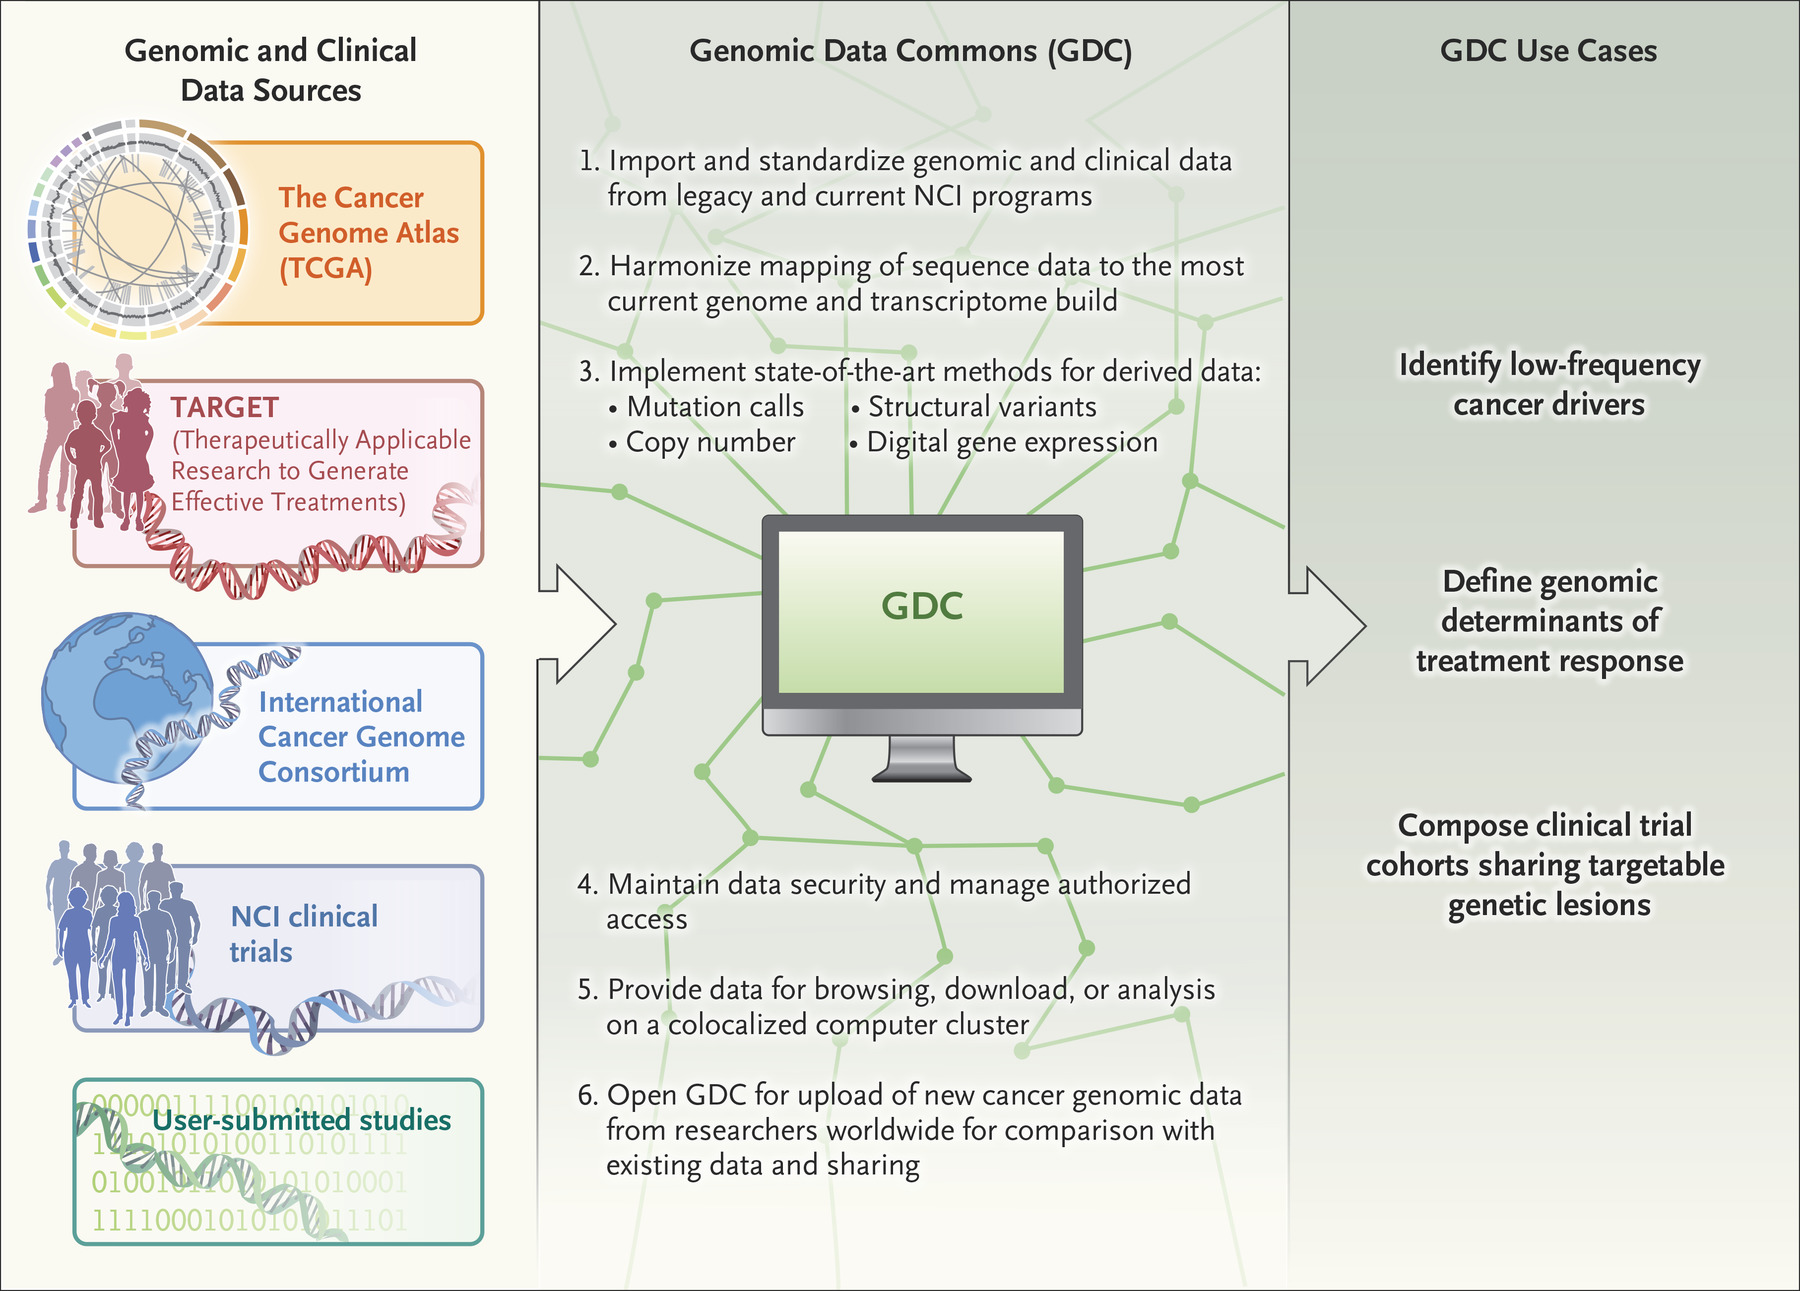
\includegraphics[width=1\textwidth]{figuras/funcionamiento_gdc.jpeg} \\
\end{center}

GDC Portal, a día 22 de Junio, contenía información sobre unos 84.000 casos, 23.000 genes y más de 3 millones de mutaciones de genes \cite{GDCPortal}. Algunos de estos datos son abiertos, mientras que para otros es necesario solicitar acceso. Los datos de los que dispone son muy variados, y se pueden distinguir en tres grandes categorías:

\begin{itemize}
	\item Información clínica, como la edad del sujeto, su sexo o el estadio del cáncer del que ha sido diagnosticado.
	\item Información genética y transcriptómica proveniente de diversos proyectos de investigación.
	\item Imágenes de tejidos tumorales y sanos.
\end{itemize} 

Para el presente trabajo se han descargado de GDC Portal todos los datos que cumplen las siguientes condiciones:

\begin{itemize}
	\item Son datos transcriptómicos del programa Cancer Genoma Atlas (TCGA), dirigido por dos organismos estadounidenses: el Instituto Nacional del Cáncer (NCI) y el Instituto Nacional para la Investigación del Genoma Humano (NHGRI) \cite{NationalCancerInstitutea}. 
	\item Contienen información sobre tumores o tejidos sanos de cáncer de hígado, o colon-recto. Se han excluido metástasis en hígado y tumores recurrentes.
	\item El tipo de estrategia experimental es RNA-Seq, y el tipo de flujo de trabajo es HTSeq - Counts.
\end{itemize}

Para cáncer de hígado se han descargado datos sobre 462 pacientes, de los cuales 404 tenían cáncer (87,4\%) y 58 estaban sanos (12,6\%).  Para cáncer de colon-recto, se han descargado datos sobre 695 pacientes: 644 con cáncer (92,7\%) y 58 sanos (7,3\%).

\subsection{Análisis}

Para el análisis se ha utilizado el software estadístico \texttt{R} \cite{R} y el paquete \texttt{KnowSeq} (v.1.1.19) \cite{KnowSeq}, librería que ha sido desarrollada por los tutores del presente trabajo, y en la que el autor ha contribuido con pequeñas actualizaciones. El paquete está además disponible en Bioconductor, la plataforma de código abierto en R más relevante para el análisis de datos de genómica y transcriptómica \cite{Gentleman2004}.\\

Para asegurar la reproducibilidad de los análisis, en el fichero \texttt{session\_info.txt} del repositorio de GitHub asociado al trabajo \cite{Redondo-Sanchez2020} se muestran todos los paquetes utilizados y sus versiones, como resultado de ejecutar \texttt{devtools::session\_info()}.\\

Todo el código de los análisis está disponible la carpeta \texttt{analisis\_higado} del repositorio de GitHub asociado al trabajo \cite{Redondo-Sanchez2020}.

\section{Características clínicas de los tumores}
 
La plataforma GDC Portal \cite{GDCPortal} permite descargar información clínica sobre los pacientes que tienen casos de cáncer, aunque no sobre los casos sanos.

\subsection{Características clínicas para cáncer de hígado}

En la Tabla 9 se muestra  la distribución de casos de cáncer de hígado según algunas variables de interés. Los casos se recogieron entre los años 1995 y 2013, con el 67,6\% de los casos recogidos entre los años 2010 y 2013. La mayoría de los casos son hombres (65,3\%) y están diagnosticados en estadios iniciales (70,3\% en estadios I y II). La edad media de diagnóstico es de 60,1 años (mediana: 61,7 años), con un rango de edad que comprende de los 16 a los 87 años. Un 5,0\% de los casos son hispanos o latinos y más de la mitad son blancos (52,5\%), que es la raza más común seguida por asiáticos (39,9\%) y negros o afroamericanos (4,7\%). Aproximadamente dos de cada tres personas estaban vivas en el momento del último contacto realizado (63,6\%).\\

\newpage
\textbf{Tabla 9}. Características clínicas de los casos de cáncer de hígado. Distribución de casos y porcentaje según sexo, edad, estadio, etnia, raza y estado vital.

\begin{table}[H]
	\centering
	\begin{tabular}{rc}
		\cline{2-2}
		\multicolumn{1}{l}{}                           & \multicolumn{1}{c}{\textbf{Número de casos (Porcentaje)}} \\ \hline
		\multicolumn{1}{l}{\textbf{Total}} & 404 (100\%)                                      \\ \hline
		\multicolumn{1}{l}{\textbf{Sexo}}              &                                                  \\
		Hombre                                         & 264 (65,3\%)                                     \\
		Mujer                                          & 140 (34,7\%)                                     \\ \hline
		\multicolumn{1}{l}{\textbf{Grupo de edad}}     &                                                  \\
		$\leq$40 años                                      & 34 (8,4\%)                                       \\
		41-50 años                                     & 40 (9,9\%)                                       \\
		51-60 años                                     & 106 (26,2\%)                                     \\
		61-70 años                                     & 127 (31,4\%)                                     \\
		71-80 años                                     & 77 (19,1\%)                                      \\
		$>$80 años                                       & 16 (4,0\%)                                         \\
		Desconocido                                    & 4 (1,0\%)                                          \\ \hline
		\multicolumn{1}{l}{\textbf{Estadio}}           &                                                  \\
		Estadio I                                      & 189 (46,8\%)                                     \\
		Estadio II                                     & 95 (23,5\%)                                      \\
		Estadio III                                    & 82 (20,3\%)                                      \\
		Estadio IV                                     & 7 (1,7\%)                                        \\
		Desconocido                                    & 31 (7,7\%)                                       \\ \hline
		\multicolumn{1}{l}{\textbf{Etnia}}             &                                                  \\
		Hispano o latino                               & 20 (5,0\%)                                         \\
		No hispano ni latino                           & 365 (90,3\%)                                     \\
		Desconocido                                    & 19 (4,7\%)                                       \\ \hline
		\multicolumn{1}{l}{\textbf{Raza}}              &                                                  \\
		Blanco                                         & 212 (52,5\%)                                     \\
		Asiático                                       & 161 (39,9\%)                                     \\
		Negro o afroamericano                          & 19 (4,7\%)                                       \\
		Desconocido                                    & 10 (2,5\%)                                       \\
		Indio americano o nativo de Alaska             & 2 (0,5\%)                                        \\ \hline
		\multicolumn{1}{l}{\textbf{Estado vital}}      &                                                  \\ 
		Vivo                                           & 257 (63,6\%)                                     \\
		Fallecido                                         & 146 (36,1\%)                                     \\
		Desconocido                                    & 1 (0,2\%)                                        \\ \hline
	\end{tabular}
\end{table}

En la Tabla 10 se muestran tablas de contingencia del estado vital según sexo, grupo de edad y estadio. Se han realizado pruebas de chi cuadrado ($\chi^2$) \cite{Pearson1900} para evaluar la independencia o no del estado vital con respecto a las distintas variables, aplicando la corrección de Yates \cite{Yates1934} cuando fue necesario. El código completo del análisis se muestra en el fichero \texttt{analisis\_higado\textbackslash03\_analisis\_datos\_clinicos.R} del repositorio de GitHub asociado al trabajo \cite{Redondo-Sanchez2020}.\\

\textbf{Tabla 10}. Características clínicas de los casos de cáncer de hígado. Distribución de casos y porcentaje según sexo, grupo de edad, estadio, etnia, raza y estado vital.

\begin{table}[H]
	\centering
	\begin{tabular}{rrrc}
		\cline{2-4}
		\multicolumn{1}{l}{}                           & \multicolumn{1}{c}{\textbf{Vivos}} & \multicolumn{1}{c}{\textbf{Fallecidos}} & \multicolumn{1}{l}{\textbf{p-valor}} \\ \hline
		\multicolumn{1}{l}{\textbf{Número de casos}} & \multicolumn{1}{c}{257}            & \multicolumn{1}{c}{146}     & \multicolumn{1}{l}{}                     \\ \hline
		\multicolumn{1}{l}{\textbf{Sexo}}              &                           &                             & 0,033                                    \\
		Hombre                                         & 178 (67,7\%)              & 85 (32,3\%)                 &                                          \\
		Mujer                                          & 79 (83,2\%)               & 16 (16,8\%)                 &                                          \\ \hline
		\multicolumn{1}{l}{\textbf{Grupo de edad}}     &                           &                             & 0,018                                    \\
		$\leq$40 años                                      & 24 (70,6\%)               & 10 (29,4\%)                 &                                          \\
		41-50 años                                     & 27 (67,5\%)               & 13 (32,5\%)                 &                                          \\
		51-60 años                                     & 68 (64,2\%)               & 38 (35,8\%)                 &                                          \\
		61-70 años                                     & 89 (70,6\%)               & 37 (29,4\%)                 &                                          \\
		71-80 años                                     & 42 (54,5\%)               & 35 (45,5\%)                 &                                          \\
		$>$80 años                                   & 5 (31,3\%)                & 11 (68,8\%)                 &                                          \\ \hline
		\multicolumn{1}{l}{\textbf{Estadio}}           &                           &                             & $<$0,001                         \\
		Estadio I                                      & 138 (73,4\%)              & 50 (26,6\%)                 &                                          \\
		Estadio II                                     & 64 (67,4\%)               & 31 (32,6\%)                 &                                          \\
		Estadio III                                    & 39 (47,6\%)               & 43 (52,4\%)                 &                                          \\
		Estadio IV                                     & 3 (42,9\%)                & 4 (57,1\%)                  &                                          \\ \hline
	\end{tabular}
\end{table}

Para las variables con datos faltantes se ha realizado un análisis de casos completos.  La mortalidad entre los casos es el doble en hombres (32,3\%) que en mujeres (16,8\%). La mortalidad aumenta conforme aumenta la edad, desde 29,4\% en menores de 41 años hasta 68,8\% en mayores de 80 años. El estadio es uno de los principales factores pronósticos del cáncer, algo que se refleja en la gran diferencia existente en la supervivencia entre estadios. En los estadios iniciales (I-II) la supervivencia está cerca al 30\% y en los más avanzados (III-IV) más cerca del 55\%. Se detecta una dependencia entre todas las variables consideradas (sexo, grupo de edad y estadio)  y el estado vital, con p-valores $<$0,05 en todos los casos.

\subsection{Características clínicas para cáncer de colon-recto}

En la Tabla 11 se muestra  la distribución de casos de cáncer de colon-recto según algunas variables de interés. Los casos se recogieron entre los años 1998 y 2013, con la mayoría de los casos recogidos entre los años 2007 y 2011. La proporción entre hombres y mujeres es similar (53,1\% y 46,9\% respectivamente), y los estadios más comunes son los intermedios (estadio II: 36,3\% y estadio III: 28,7\%). La edad media de diagnóstico es de 66,7 años (mediana: 68,1 años), con un rango de edad de entre 31 y 90 años. Aproximadamente la mitad de los pacientes son blancos (47,3\%), que es la raza más común seguida por negros o afroamericanos (10,5\%) y asiáticos (2,1\%). Se desconoce la raza del 40,0\% de las personas. Aproximadamente cuatro de cada cinco personas estaban vivas en el momento del último contacto realizado (79,2\%), y sólo un 0,8\% de los casos son hispanos o latinos.\\

\newpage
\textbf{Tabla 11}. Características clínicas de los casos de cáncer de colon-recto. Distribución de casos y porcentaje según sexo, edad, estadio, etnia, raza y estado vital.

\begin{table}[H]
		\centering
	\begin{tabular}{rr}
		\cline{2-2}
		\multicolumn{1}{l}{}                       & \multicolumn{1}{c}{\textbf{Número de casos (Porcentaje)}} \\ \hline
		\multicolumn{1}{l}{\textbf{Total}}         & 620 (100\%)                                               \\ \hline
		\multicolumn{1}{l}{\textbf{Sexo}}          &                                                           \\
		Hombre                                     & 329 (53,1\%)                                              \\
		Mujer                                      & 291 (46,9\%)                                              \\ \hline
		\multicolumn{1}{l}{\textbf{Grupo de edad}} &                                                           \\
		$\leq$40 años                                   & 16 (2,6\%)                                                \\
		41-50 años                                 & 59 (9,5\%)                                                \\
		51-60 años                                 & 101 (16,3\%)                                              \\
		61-70 años                                 & 173 (27,9\%)                                              \\
		71-80 años                                 & 171 (27,6\%)                                              \\
		$>$80 años                               & 98 (15,8\%)                                               \\
		Desconocido                                & 2 (0,3\%)                                                 \\ \hline
		\multicolumn{1}{l}{\textbf{Estadio}}       &                                                           \\
		Estadio I                                  & 105 (16,9\%)                                              \\
		Estadio II                                 & 225 (36,3\%)                                              \\
		Estadio III                                & 178 (28,7\%)                                              \\
		Estadio IV                                 & 89 (14,4\%)                                               \\
		Desconocido                                & 23 (3,7\%)                                                \\ \hline
		\multicolumn{1}{l}{\textbf{Etnia}}         &                                                           \\
		Hispano o latino                           & 5 (0,8\%)                                                 \\
		No hispano ni latino                       & 352 (56,8\%)                                              \\
		Desconocido                                & 263 (42,4\%)                                              \\ \hline
		\multicolumn{1}{l}{\textbf{Raza}}          &                                                           \\
		Blanco                                     & 293 (47,3\%)                                              \\
		Asiático                                   & 13 (2,1\%)                                                \\
		Negro o afroamericano                      & 65 (10,5\%)                                               \\
		Desconocido                                & 248 (40\%)                                                \\
		Indio americano o nativo de Alaska         & 1 (0,2\%)                                                 \\ \hline
		\multicolumn{1}{l}{\textbf{Estado vital}}  &                                                           \\
		Vivo                                       & 491 (79,2\%)                                              \\
		Muerto                                     & 129 (20,8\%)                                              \\ \hline
	\end{tabular}
\end{table}

En la Tabla 12 se muestran tablas de contingencia del estado vital según sexo, grupo de edad y estadio. Se han realizado pruebas de chi cuadrado ($\chi^2$) \cite{Pearson1900} para evaluar la independencia o no del estado vital con respecto a las distintas variables, aplicando la corrección de Yates \cite{Yates1934} cuando fue necesario. El código completo del análisis se muestra en el fichero \texttt{analisis\_cr\textbackslash03\_analisis\_datos\_clinicos.R} del repositorio de GitHub asociado al trabajo \cite{Redondo-Sanchez2020}.\\

\textbf{Tabla 12}. Características clínicas de los casos de cáncer de colon-recto. Distribución de casos y porcentaje según sexo, grupo de edad, estadio, etnia, raza y estado vital.

\begin{table}[H]
		\centering
	\begin{tabular}{rrrc}
		\cline{2-4}
		\multicolumn{1}{l}{}                           & \multicolumn{1}{c}{\textbf{Vivos}} & \multicolumn{1}{c}{\textbf{Fallecidos}} & \multicolumn{1}{c}{\textbf{p-valor}} \\ \hline
		\multicolumn{1}{l}{\textbf{Número de tumores}} & 491            & 129                 &                  \\ \hline
		\multicolumn{1}{l}{\textbf{Sexo}}              &                &                     & 0,993            \\
		Hombre                                         & 260 (79\%)     & 69 (21,0\%)           &                  \\
		Mujer                                          & 231 (79,4\%)   & 60 (20,6\%)         &                  \\ \hline
		\multicolumn{1}{l}{\textbf{Grupo de edad}}     &                &                     & \textless{}0,001 \\
		$\leq$40 años                                     & 14 (87,5\%)    & 2 (12,5\%)          &                  \\
		41-50 años                                     & 51 (86,4\%)    & 8 (13,6\%)          &                  \\
		51-60 años                                     & 85 (84,2\%)    & 16 (15,8\%)         &                  \\
		61-70 años                                     & 150 (86,7\%)   & 23 (13,3\%)         &                  \\
		71-80 años                                     & 120 (70,2\%)   & 51 (29,8\%)         &                  \\
		$>$80 años                                  & 70 (71,4\%)    & 28 (28,6\%)         &                  \\ \hline
		\multicolumn{1}{l}{\textbf{Estadio}}           &                &                     & \textless{}0,001 \\
		Estadio I                                      & 98 (93,3\%)    & 7 (6,7\%)           &                  \\
		Estadio II                                     & 192 (85,3\%)   & 33 (14,7\%)         &                  \\
		Estadio III                                    & 139 (78,1\%)   & 39 (21,9\%)         &                  \\
		Estadio IV                                     & 48 (53,9\%)    & 41 (46,1\%)         &                  \\ \hline
	\end{tabular}
\end{table}

Para las variables con datos faltantes se ha realizado un análisis de casos completos (exclusión del análisis de los casos con tenían datos faltantes).  La mortalidad es muy similar en hombres y mujeres, sin diferencias significativas (p-valor: 0,993). Se detecta una dependencia entre el estado vital con las variables de grupo de edad y estadio, con p-valores $<$0,001. En mayores de 70 años la mortalidad está cerca del 30\%, el doble de la mortalidad existente en otros grupos de edad. Hay grandes diferencias de mortalidad en función del estadio diagnosticado, que pasa del 6,7\% en el estadio I al 46,1\% en el estadio IV.

\section{Resultados de clasificación biclase para cáncer de hígado}

\subsection{Entrenamiento de modelo}

\subsection{Validación en test}

\section{Resultados de clasificación multiclase para cáncer de hígado}

\section{Resultados de clasificación biclase para cáncer de colon-recto}

\textcolor{red}{Completar una vez esté depurado el análisis de cáncer de hígado.}

\section{Resultados de clasificación multiclase para cáncer de colon-recto}

\textcolor{red}{Completar una vez esté depurado el análisis de cáncer de hígado.}

\section{Conclusiones}

\textcolor{red}{Interpretar resultados con cautela: ver pág. 65 de \cite{CastilloSecilla2020} (referencias 77-79).}\\

	
	% Aplicación web para detección de biomarcadores
	\chapter{\texttt{biomarkeRs}: una aplicación web interactiva para detección de biomarcadores}

\textcolor{red}{La aplicación ya está traducida al inglés, y he implementado transiciones de carga como propuso Daniel. La desarrollaré completamente en Agosto.}\\

\textcolor{red}{Capítulo por escribir, podéis pasar al siguiente porque sólo hay notas sobre lo que puedo escribir.}

\section{Desarrollo de la aplicación}

\textcolor{red}{\texttt{Shiny}, versión, documentación breve sobre Shiny, reactividad, incluye CSS, comentar que es accesible a todo el mundo (Shiny Server, o shinyapps.io), subir a una URL y compartir...}.\\

El fichero \texttt{shiny\textbackslash app.R} del repositorio de GitHub asociado al trabajo \cite{Redondo-Sanchez2020}  contiene el código de R desarrollado para crear la aplicación web.

\section{Utilidades de la aplicación}

\textcolor{red}{Útil para realizar análisis genéticos para personas sin apenas conocimientos previos de programación. Capturas de pantalla con ejemplos. Escribir pequeño manual de uso. Quizá grabar vídeo mostrando la aplicación (y subir GIF a README del repositorio de GitHub).}
	
	% Conclusiones y líneas abiertas de trabajo
	\chapter{Conclusiones y líneas abiertas de trabajo}

\textcolor{red}{\texttt{KnowSeqWeb}, interfaz web para acercar el uso de KnowSeq a personas sin conocimientos de programación. Resaltar diferencias entre KnowSeqWeb y biomaRcadores: multiclase/biclase, sin preprocesamiento/con, proceso automático/guiado con más capacidad de decisión, ...}


	
	% Bibliografía
	\newpage
	\phantomsection
	\addcontentsline{toc}{chapter}{Bibliografía}
	\bibliographystyle{unsrt}
	\thispagestyle{empty}
	\bibliography{bibliografia}
	
	% Apéndices
	\appendix
	\backmatter
	\chapter{Anexo I: Código de análisis en R}
	\section*{Anexo I: Código de análisis en \texttt{R}}\label{anexo1}

\subsection*{Información sobre la sesión en \texttt{R}: paquetes y versiones}

\textbf{Caja 1}. Resultado de \texttt{devtools::session\_info()} tras realizar los análisis.

\lstinputlisting{codigo/session_info.txt}

\subsection*{Análisis para cáncer de hígado}

\textbf{Caja XX}. Código en \texttt{R} del análisis realizado para cáncer de hígado.

\lstinputlisting[language=R]{codigo/cabecera.R}

	\chapter{Anexo II: Código de aplicación web}
	\section*{Anexo II: Código de aplicación web}\label{anexo2}

\subsection*{Funciones}

\textbf{Caja XX}. Definición de \texttt{funcion}.

\lstinputlisting[language=R]{codigo/cabecera.R}
		
\end{document}